\documentclass[journal]{IEEEtran}



\usepackage{makeidx}  % allows for indexgeneration
\usepackage{url}
\usepackage{mathrsfs}
\usepackage{graphicx}
\usepackage{indentfirst}
\usepackage{amsfonts}
\usepackage{amsmath}
\usepackage{amssymb}
\usepackage{fancyhdr}
\usepackage{subfigure}
\usepackage{stmaryrd}
\usepackage{cite}
\usepackage{color}
\usepackage{overpic}
\usepackage{amsfonts,amsmath,amssymb}
\usepackage{dblfloatfix}
\usepackage[hidelinks]{hyperref}



%

% \usepackage{caption}
% \usepackage{subcaption}
\usepackage[utf8]{inputenc}


\newcommand{\abs}[1]{\lvert#1\rvert}
\newcommand{\norm}[1]{\lVert#1\rVert}
\newcommand{\todo}[1]{\textcolor{red}{\footnotesize \textsf{#1}}}
\newcommand{\R}{\mathbb{R}}
\DeclareMathOperator{\sgn}{sgn}




\graphicspath{{Figures/}}

% list here all the paths to your figure folders

\hyphenation{op-tical net-works semi-conduc-tor un-te-the-red intra-ocular mi-cro-ro-bots O-cto-Mag}

\makeindex

\title{\LARGE \bf
Achieving Commutation Control of an MRI-powered Robot Actuator
}

\author{Ouajdi Felfoul, 
Aaron Becker,~\IEEEmembership{Member,~IEEE}, 
Christos Bergeles,~\IEEEmembership{Member,~IEEE}, \\
and Pierre E. Dupont,~\IEEEmembership{Fellow,~IEEE}%
\thanks{O.\ Felfoul, and P.~E.~Dupont are with the Department of Cardiovascular Surgery, Boston Children's Hospital, Harvard Medical School, 02115 Boston, Massachusetts {\tt\small \{firstname.lastname@childrens.harvard.edu\}}.
 A.~Becker is now with the University of Houston, Houston TX, 77204-4005 {\tt\small \{atbecker@uh.edu\}}.
C.~Bergeles is now with the Hamlyn Centre, Imperial College London, London SW7 2AZ, U.K. {\tt\small \{c.bergeles@imperial.ac.uk\}}.
}%
\thanks{This work was supported by the National Science Foundation under grant IIS-1208509 and by the Wyss Institute for Biologically Inspired Engineering. Parts of this research have appeared at the 2013 IEEE Int. Conf. Robotics and Automation \cite{bergeles2013closed}.}
\thanks{Manuscript received April 19, 2014; revised January 27, 2015.}}



\begin{document}

\maketitle

\begin{abstract}
Actuators that are powered, imaged and controlled by Magnetic Resonance ({MR}) scanners could inexpensively provide wireless control of MR-guided robots. Similar to traditional electric motors, the MR scanner acts as the stator and generates propulsive torques on an actuator rotor containing one or more ferrous particles. Generating maximum motor torque while avoiding instabilities and slippage requires closed-loop control of the electromagnetic field gradients, i.e., \emph{commutation}. Accurately estimating the position and velocity of the rotor is essential for high-speed control, which is a challenge due to the low refresh rate and high latency associated with MR signal acquisition. This paper proposes and demonstrates a method for closed-loop commutation based on interleaving pulse sequences for rotor imaging and rotor propulsion. This approach is shown to increase motor torque and velocity, eliminate rotor slip and enable regulation of rotor angle. Experiments with a closed-loop MRI actuator produced a maximum force of 9.4N.
\end{abstract}

\section{Introduction}
\label{sec:introduction}
\IEEEPARstart{M}{agnetically} actuated devices are an emerging class of tools for both diagnostic and interventional medical procedures. For example, endoscopes actuated by permanent magnets have been proposed for imaging the GI tract \cite{tognarelli2012magnetic} and the stomach \cite{yim2012design}. Catheters with embedded current-carrying micro-coils have been actuated by the forces generated by the magnetic field of the MRI scanner \cite{Cenk2014Catheter}. Custom electromagnetic control systems have been employed for intravascular \cite{yu2010novel}, intraocular \cite{ulrich2013mobility} and intracochlear \cite{clark2012magnetic} microrobot navigation. These magnetic actuation platforms require coupling to an imaging system, such as ultrasound \cite{tognarelli2012magnetic}, fluoroscopy \cite{yu2010novel}, or surgical microscopy \cite{ulrich2013mobility}.

Since MRI delivers high amounts of non-ionizing electromagnetic energy, scanners offer the potential for both electromagnetic energy transfer as well as imaging. Examples of this approach include an MR-powered swimming endoscope \cite{kosa2012mri} and an intravascular swimming robot \cite{chanu2008adapting} \cite{mathieu2006method}. In \cite{kosa2012mri}, undulating motion is generated through interaction between the static magnetic field of the scanner and an electric-current-induced magnetic field in a coiled tail. Alternatively, in \cite{chanu2008adapting} \cite{mathieu2006method} magnetic gradients, normally used for MR-signal spatial encoding, are exploited to induce forces in ferromagnetic material and so to propel an intravascular robot.

Centimeter-scale MRI-powered and imaged robots would be small enough to fit inside the bore to access hard-to-reach mid-torso locations or could even fit inside the body. While a variety of MR-compatible robots for surgical procedures ranging from brachytherapy, needle-biopsy to heart surgery have been developed\cite{song2011robotic, su2012mri, navkar2012visual, Schouten2012Biopsy, Beyersdorff2005MR, Stoianovici2014MRI, Yiallouras2014MR}, they all require actuators of high cost or high complexity and also necessitate either mechanical or electrical tethering to external control systems. 

\begin{figure}[t]
\begin{center}
	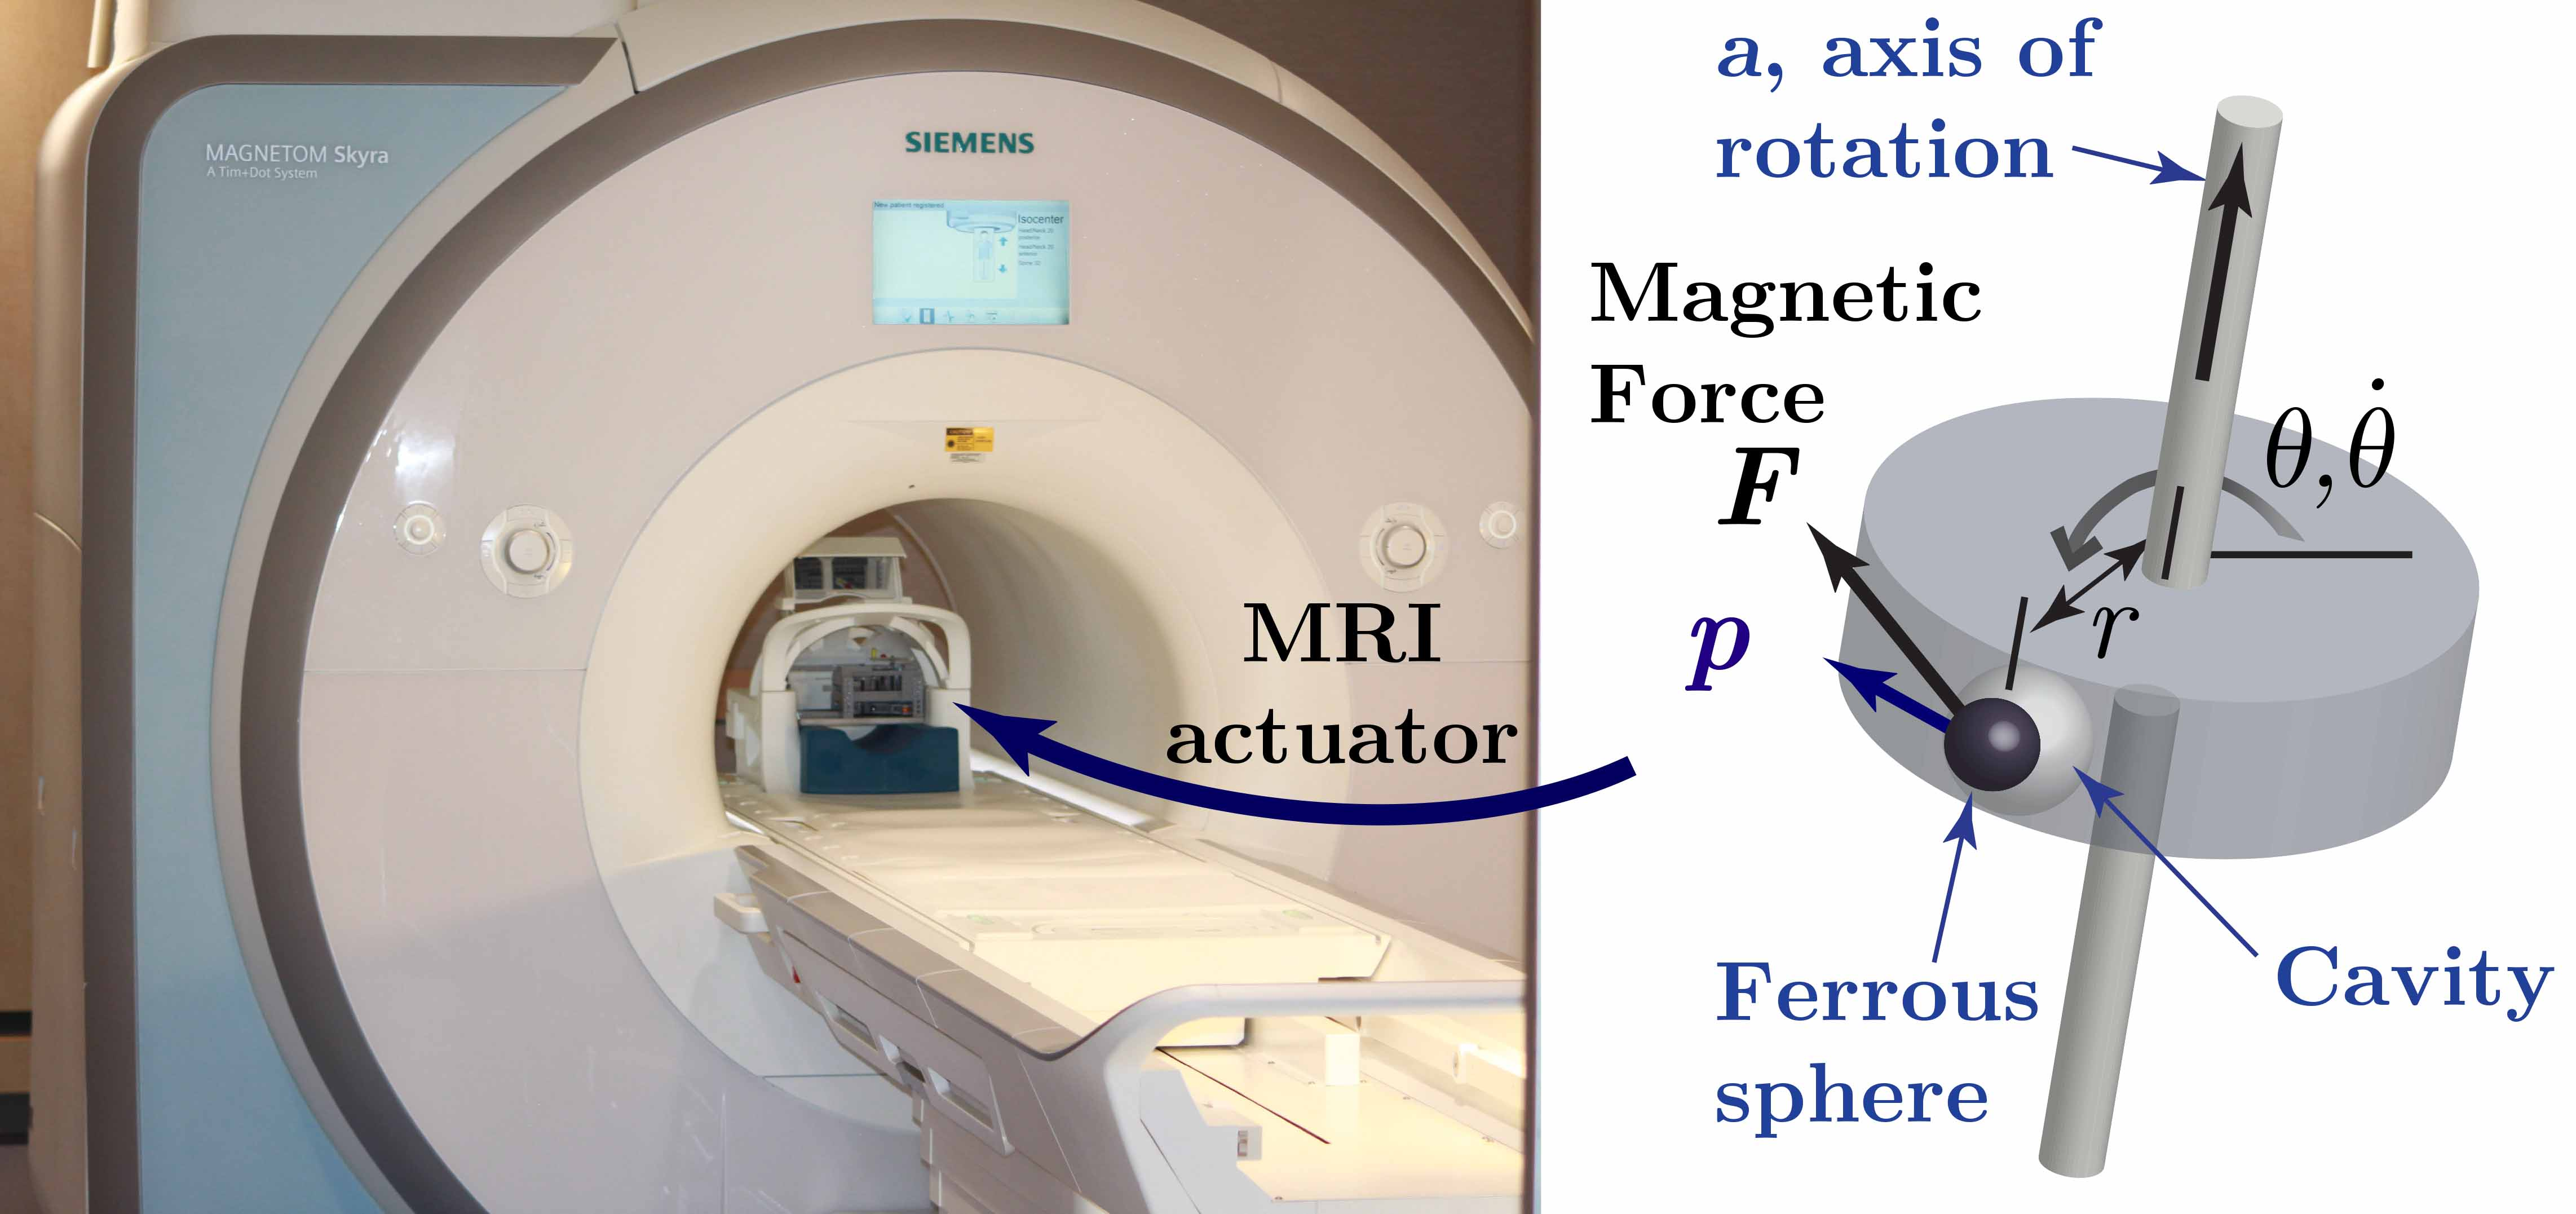
\includegraphics[width=0.95\columnwidth]{Figure1.jpg}
\end{center}
\caption{Concept of an MRI-powered actuator. Interleaved imaging and propulsion pulse sequences are used to track rotor angle and generate magnetic-gradient-based forces enabling control of both motor position and torque.
\label{fig:actuator-illustration}}
\vspace{-10pt}
\end{figure}

Alternatively, MRI-powered actuators may be fabricated inexpensively from plastic parts and metal spheres and can be actuated, imaged, and controlled directly by the MRI scanner \cite{vartholomeos2011mripowered,vartholomeos2013mri}. This approach can be explained by analogy to an electric motor, as shown in Fig.\ \ref{fig:actuator-illustration}. The scanner and the chassis of the actuator comprise the stator. A rotor with an encapsulated ferrous sphere placed inside the scanner bore is the rotational part of the actuator. Rotating MRI gradients generate forces on the ferrous sphere, which causes rotor motion. Since the sphere is enclosed in a cavity, it is free to remain aligned with the scanner's $\vec{B}_0$ field during rotor rotation. 

In our initial implementation of an MRI-powered actuator, commutation was performed in open loop using  sinusoidal gradients commanded to rotate at the desired angular rate of the motor\cite{vartholomeos2011mripowered,vartholomeos2013mri}. While this approach enabled needle insertion using an outer position control loop, it possessed several limitations. For example, load perturbations would cause the rotor to slip such that the needle would stop moving for one or more revolutions of the magnetic gradients. In addition, since the angle between the rotor and the magnetic force was not regulated, the actuator produced less torque. Finally, since position control was based on sensed needle position rather than rotor angle (at transmission input), displacement resolution was significantly reduced.

Closed-loop commutation was introduced in a conference version of this paper~\cite{bergeles2013closed}. Real-time feedback was achieved using a socket-based 3rd-party protocol \emph{RTHawk}~\cite{santos2004flexible} compatible with GE scanners. No state estimator was employed and, given the interleaving of imaging and actuation, this meant that the gradient force direction was constant between imaging sequences---implicitly assuming the rotor is stationary. While this approach was superior to open-loop commutation, performance was characterized by large commutation angle errors. 

The contributions of this paper beyond those of \cite{bergeles2013closed} are as follows. First, a state estimator is introduced that enables accurate variation of gradient force direction during execution of actuation pulse sequences. State estimates are updated using measured rotor position together with measurement noise calculated from each MRI image. Second, all pulse sequences have been redesigned to avoid the need for 3rd party software. The sequences have been implemented using the native real-time environment provided by Siemens scanners and tested on a Siemens 3T Skyra scanner. Consequently, results in this paper can be replicated on any similar Siemens scanner without the need for additional software. A third contribution of this paper is that it employs fast spin echo sequences for rotor tracking instead of gradient echo sequences. This approach provides better performance at high rotor angular velocities and in the presence of magnetic inhomogeneities \cite{Posse1990Susceptibility}. 

Furthermore, a new actuator design is presented that produces over 9N of force compared to a maximum of 0.7N as reported in \cite{bergeles2013closed}. All of the experimental results are new and include examining the effects of sampling rate and rotor velocity on tracking accuracy and imaging noise. Maximum torque is measured as a function of actuation duty cycle and is compared with the maximum torque that can be achieved in open-loop operation. In addition, new position control experiments are presented.

The paper is arranged as follows. Section \ref{sec:actuator-technology} defines the problem of MRI-based commutation. Section III presents our approach for rotor tracking based on RF-selective excitation. (Note that rotor tracking is completely independent of tissue imaging. The effect of the actuator on tissue imaging is addressed in the final subsection of Section \ref{sec:experiments}.) Section \ref{sec:gradient-control} details design of the pulse sequences needed for closed-loop rotor control while Section \ref{sec:controlLaw} presents the state estimator and controller.
Experimental validation is provided in Section \ref{sec:experiments} and conclusions appear in Section \ref{sec:conclusions}.  


\section{MRI-based Commutation}
\label{sec:actuator-technology}

An MRI scanner can apply magnetic forces to a rotor.  To maximize torque, these forces should always be directed perpendicular to the rotor. This is called \emph{commutation control}. Brushless electric motors use encoders to produce the maximum torque via commutator control, as shown in Fig.\ \ref{fig:traditional-commutator}. The current in each electromagnet is controlled based on the Hall sensors' rotor angle estimation. The forces, $F$, generated on the rotor's permanent magnet by the electromagnets should be directed such that maximum torque is generated for all angular configurations of the rotor, i.e. the angle $\psi$ in Fig.\ \ref{fig:traditional-commutator} should be $90^\circ$. The goal of commutator control is to regulate $\psi$ to this optimal value. 

There are several challenges to MRI-based commutation. In contrast to brushless electric motors where the stator's position can be sampled at high rates, the MRI position refresh rate is low. This low refresh rate has three primary causes. First, the same gradient coils are shared between actuation and imaging. Second, the imaging phase requires a minimum time to manipulate the hydrogen spins before an image can be collected. Third, following an imaging cycle, the hydrogen spins responsible for signal generation must relax before they can be excited again, imposing a minimum delay between rotor imaging. 

MRI actuation technology is also affected by latencies necessary to process imaging data and to apply the following gradient inputs. Furthermore, accurate rotor angle position measurement requires two perpendicular line scans and must account for the time delay between these scans. Finally, 
due to the low position refresh rate, the velocity measurement has low accuracy. 

As with electric motors, MRI-based commutator control maximizes torque generation and enables rotor angle control. To address the challenges of closed-loop commutation described above, three components are needed. First, a method is needed for fast imaging of the ferromagnetic rotor in air. Second, a pulse sequence must be developed that provides for real-time control of rotor angle. Third, an estimator and controller are needed that can accommodate interleaved actuation and imaging. Solutions to these components are presented in the next three sections.

\begin{figure}[t]
\begin{center}
	\subfigure[]{
		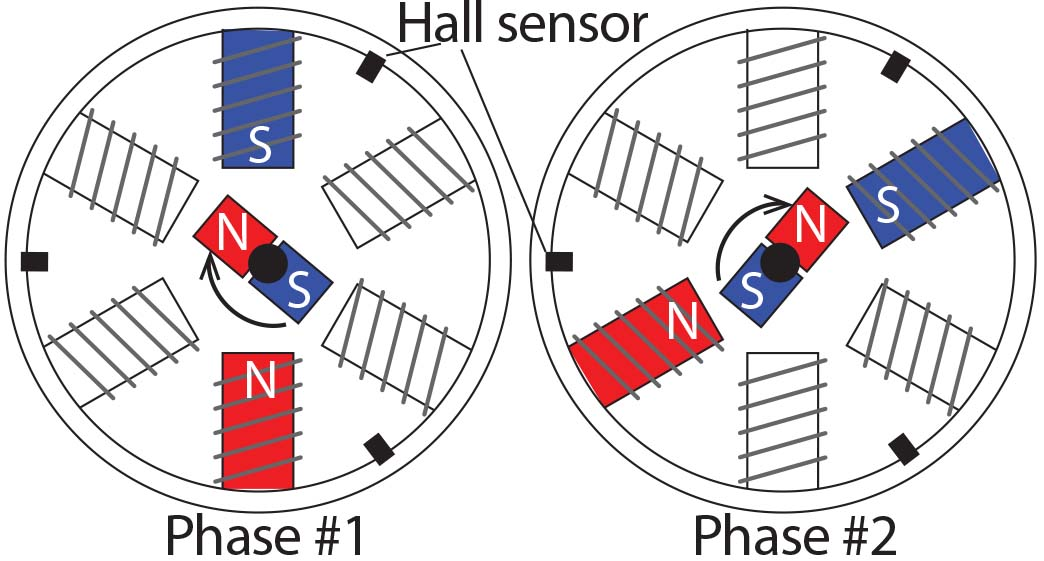
\includegraphics[width=0.47\columnwidth]{Figure2a.jpg}
		\label{fig:traditional-commutator}
	}\subfigure[]{
	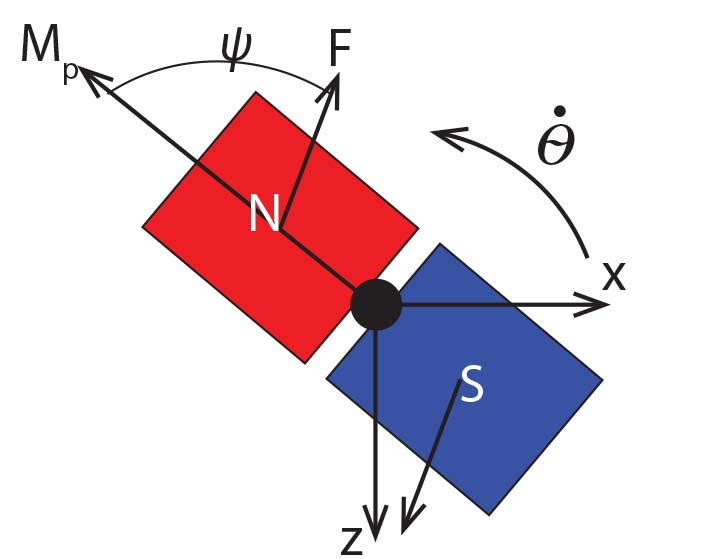
\includegraphics[width=0.47\columnwidth]{Figure2b.jpg}
		\label{fig:actuator-commutator}
	}
\end{center}
\caption{Brushless DC motor. (a) Active electromagnets during rotor motion for two consecutive configurations. (b) Rotor forces $F$, and angle $\psi$.}
\vspace{-10pt}
\end{figure}

\section{Rotor Tracking}
\label{sec:tracking}
In designing a tetherless MRI-powered actuator, the usual techniques used in MRI-based tracking are not directly applicable. For example, active tracking using small receiver coils tuned to the scanner's RF frequency \cite{qin2012prospective} require cabling and present the challenge of avoiding cable windup on the rotor. While passive tracking using fiducial markers is often an excellent approach \cite{thormer2012simultaneous}, any nearby ferromagnetic material acts as a `negative' fiducial, creating a signal void in its vicinity \cite{busse2007method}. Consequently, the ferromagnetic material needed to propel the rotor tends to neutralize any fiducial marker that is also mounted on the rotor. 

\begin{figure}
\begin{center}
	\subfigure[]{
		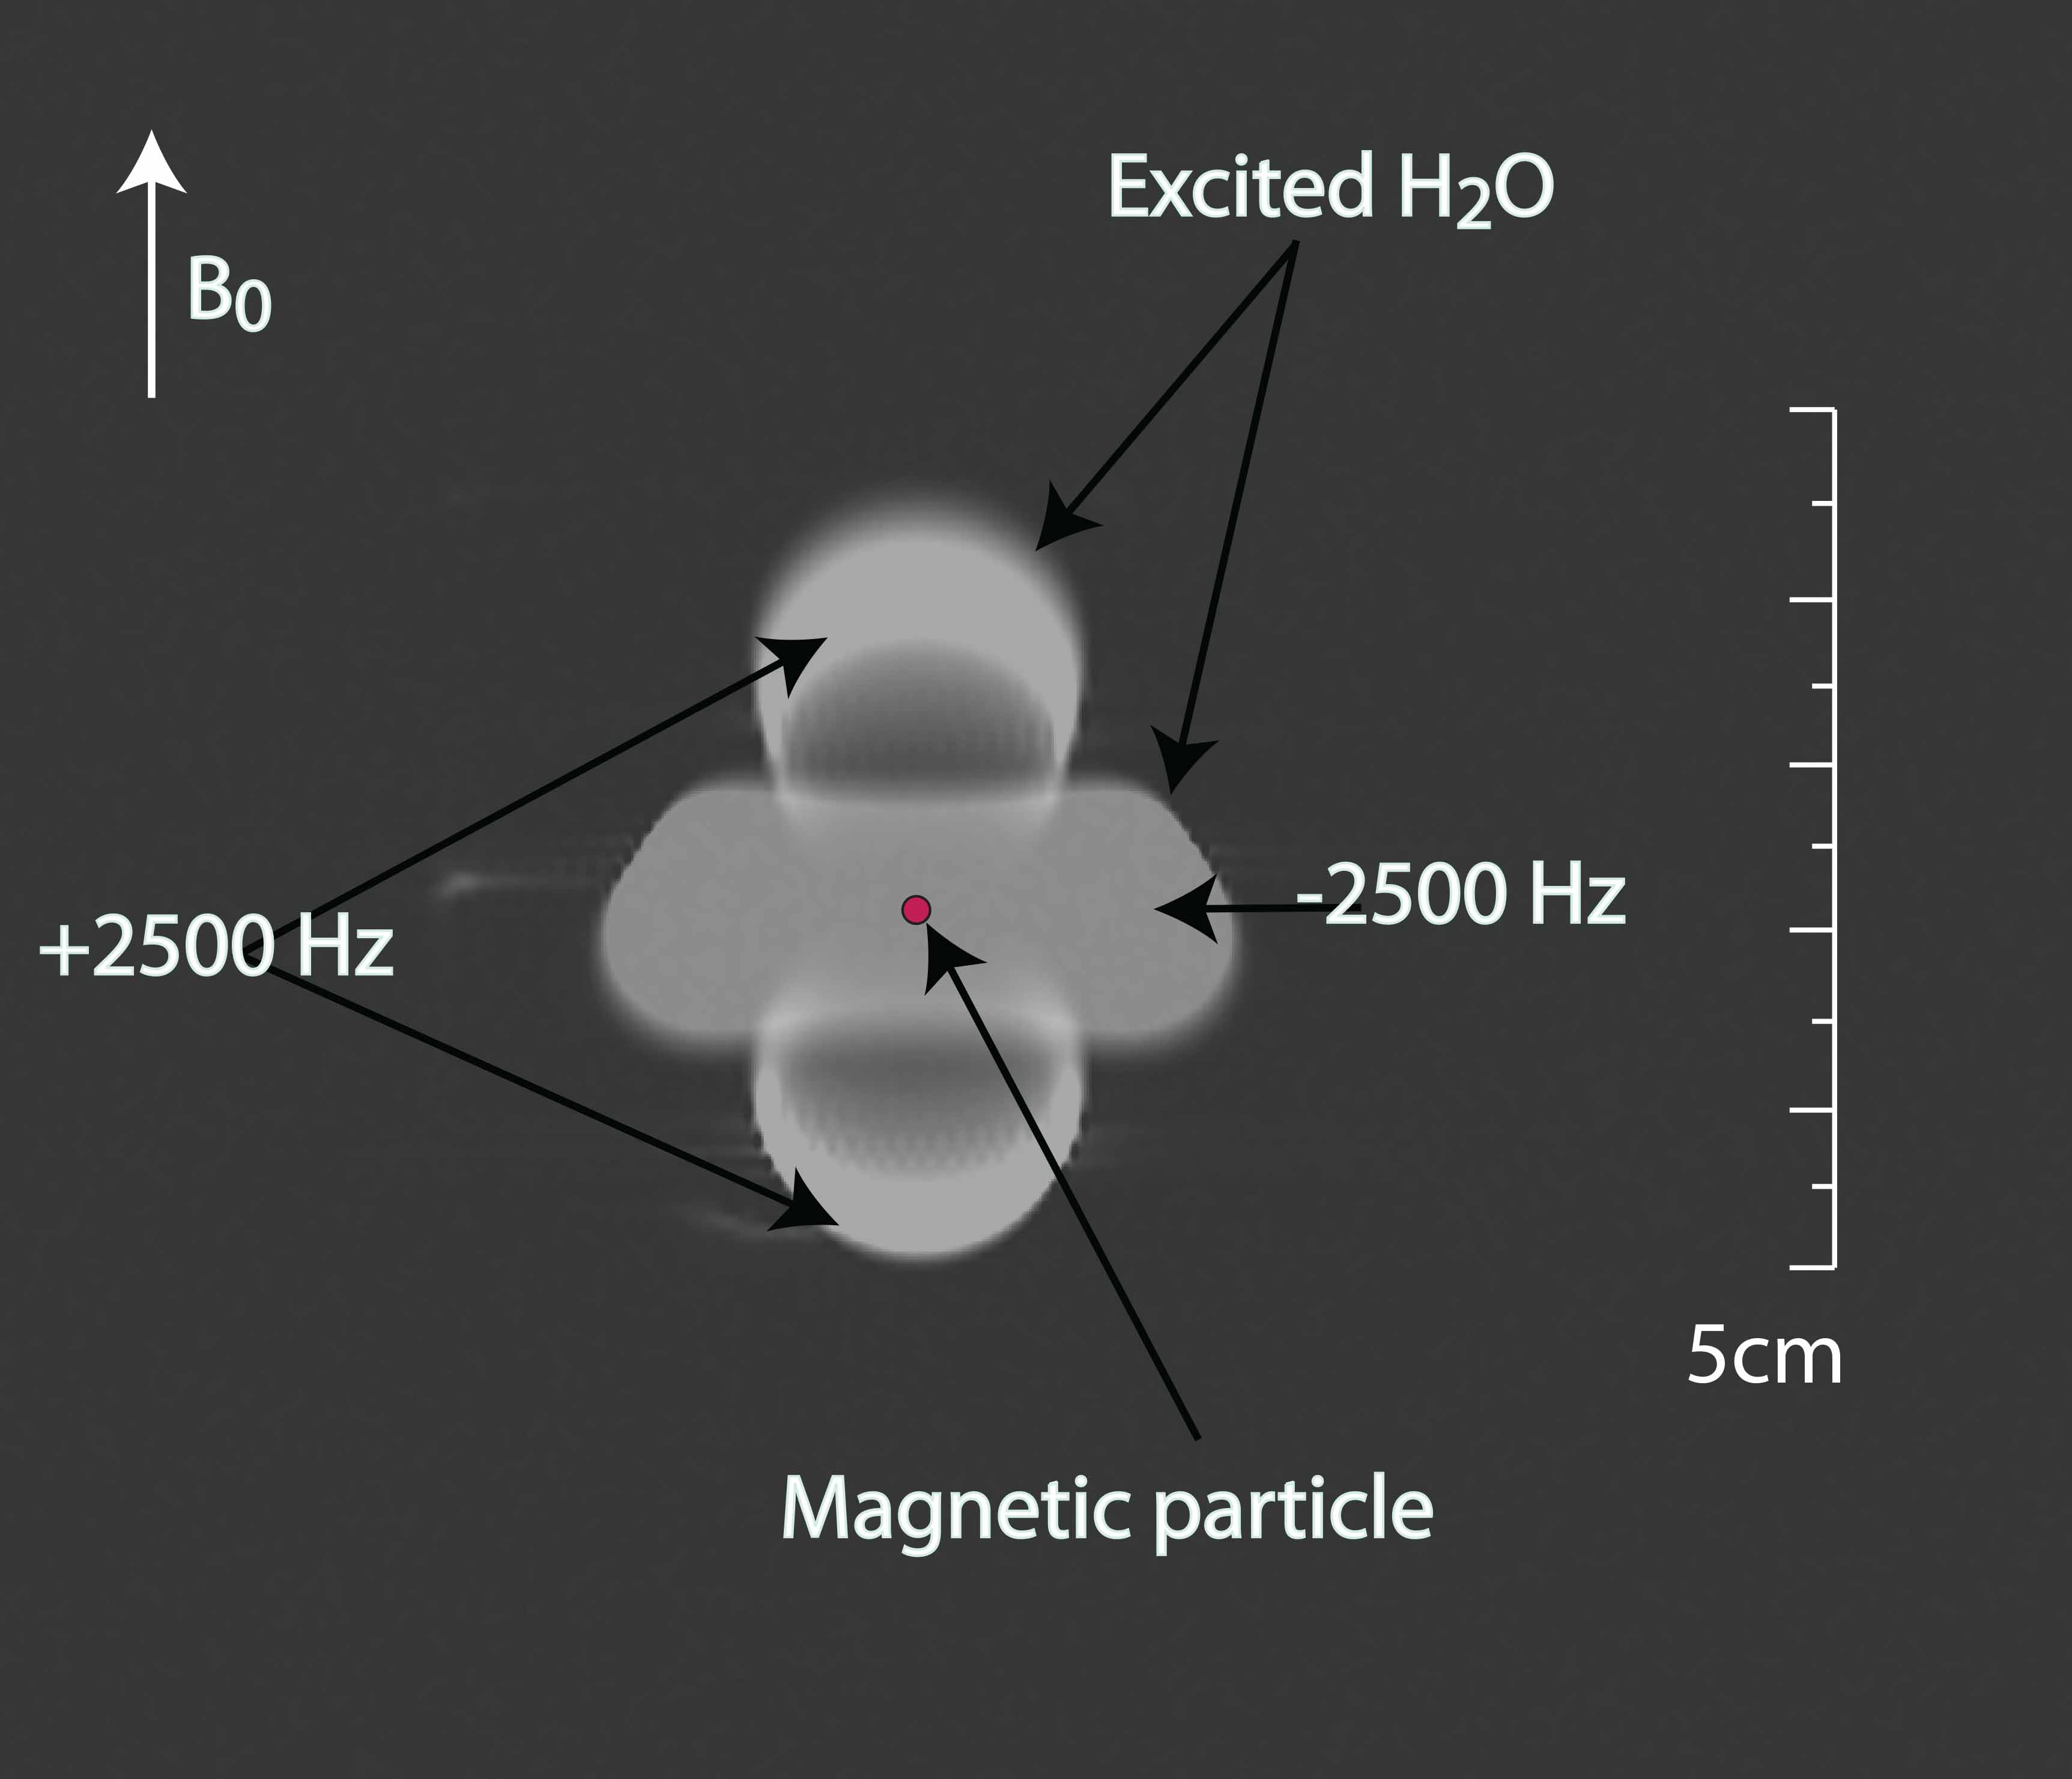
\includegraphics[width=0.47\columnwidth]{Figure3a.jpg}
		\label{fig:mss-excitation}
	}\subfigure[]{
		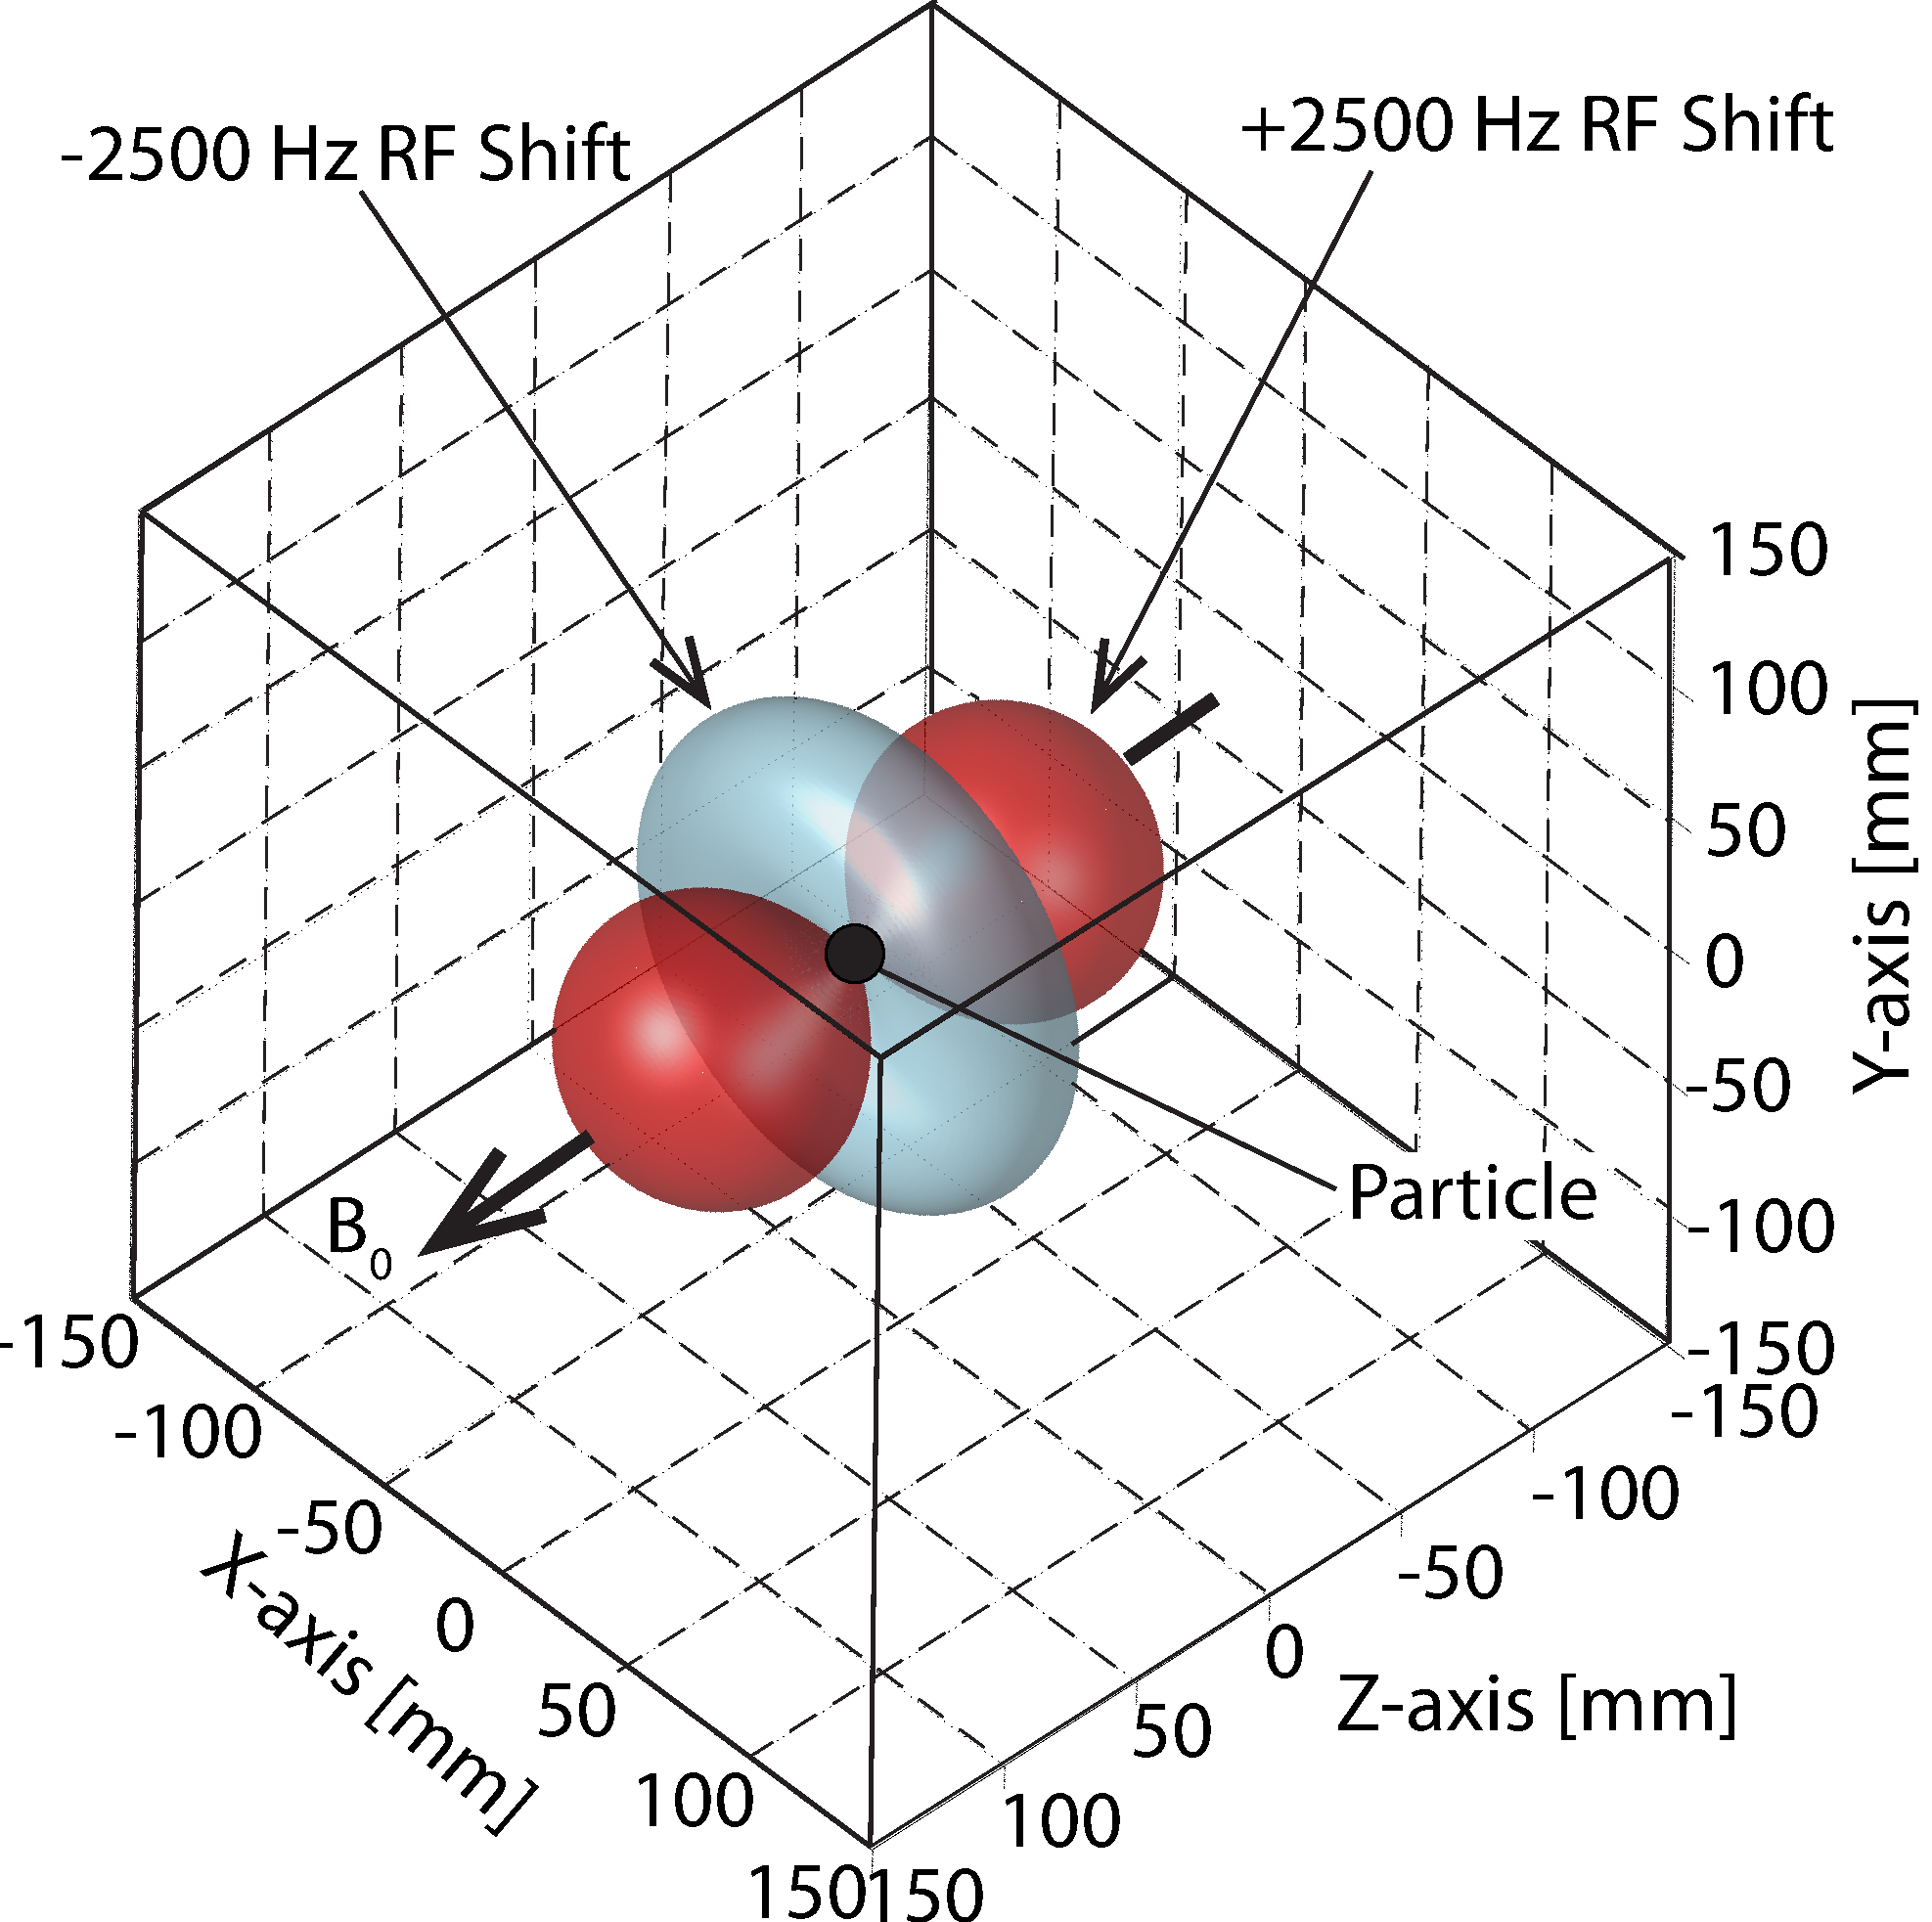
\includegraphics[width=0.47\columnwidth]{Figure3b.pdf}
		\label{fig:mss-3d}
	}
\end{center}
\caption{RF selective excitation. (a) Two superimposed MRI images using positive and negative RF-selective excitation for a 1mm radius magnetic particle. (b) Simulation of the excited region for RF pulses shifted below and above the Larmor frequency.}
\end{figure}

Recently, \cite{chanu2008adapting, cunningham2005positive} demonstrated the use of ferromagnetic particles as positive markers located inside tissue [see Fig.\ \ref{fig:mss-excitation}]. Instead of using RF pulses that correspond to the Larmor frequency of hydrogen in the presence of $\vec{B_0}$, the RF pulse frequency is selected to affect molecules that are in the $\vec{B_0} + \vec{B_p}$ field, where $\vec{B_p}$ is created by the ferrous particle. In this way, only water molecules in the vicinity of the ferromagnetic particle are excited (RF-selective excitation). By varying the RF frequency and bandwidth, different regions around the particle can be selected for excitation. Fig.\ \ref{fig:mss-3d} shows an example of the excited regions for RF frequencies above and below the Larmor frequency. Any hydrogen atoms located in the the excited region will appear brightly in an image. 

To enable rotor tracking, a new method is introduced that uses RF-selective excitation in combination with a passive fiducial marker. In this approach, the ferrous particle of the rotor excites regions similar in shape to those of Fig.\ \ref{fig:mss-3d} inside the actuator. These regions are small enough that they do not extend into the tissue surrounding the actuator. Consequently, an image taken in this way (without a fiducial marker) would be empty. 

To track the rotor, a fiducial marker is positioned on the rotor such that it is located within the excited region (specific to the  selected RF frequency and bandwidth) for all possible rotation angles. With the marker in place, an image taken using RF-selective excitation will now show only the marker since the tissue lies outside the excited region and the actuator itself is invisible since it does not contain hydrogen atoms. Since only the marker appears in the image, simple image processing can be used to determine rotor angle.

\subsection{RF Frequency and Bandwidth Selection}

Fig.\ \ref{fig:actuator-prototype} depicts the rotor showing both the ferrous sphere and the fiducial marker. The displacement of the marker relative to the sphere is given by the radial displacement, $r_d$ and the vertical displacement, $\textnormal{v}_d$. Note that a displacement in the third relative coordinate direction is not considered here since its effect would be equivalent to the radial displacement as the rotor rotates with respect to candidate RF-excited regions [see Fig. \ref{fig:mss-3d}].

\begin{figure}
\begin{center}
	\subfigure[]{
		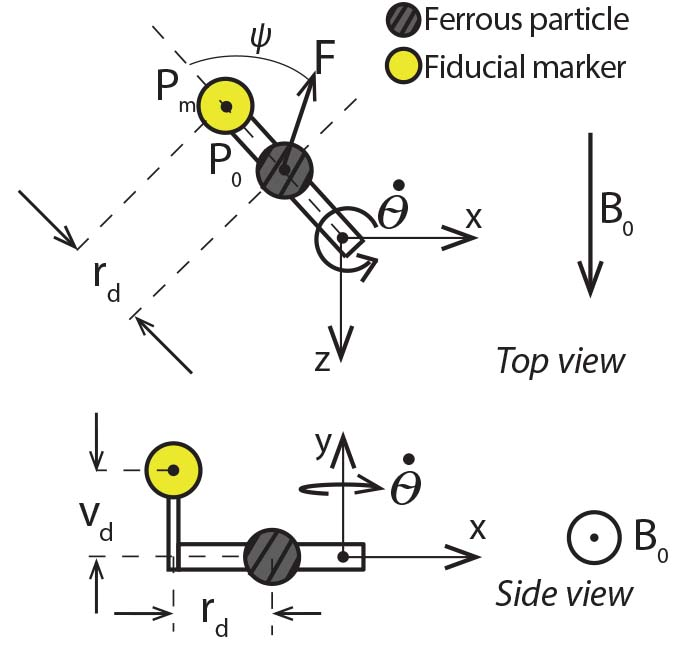
\includegraphics[width=0.44\columnwidth]{Figure4a.jpg}
		\label{fig:actuator-prototype}
	}
	\subfigure[]{
		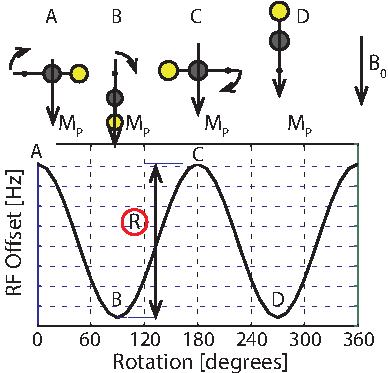
\includegraphics[width=0.44\columnwidth]{Figure4b.pdf}
		\label{fig:rf-example}
	}
\end{center}
\caption{Locating RF-selective fiducial marker on rotor. (a) Top view and side view of rotor. (b) Marker configuration example with $v_d=0$ that requires configuration-dependent RF frequency to image marker.  Rotor configurations of $0^\circ$, $90^\circ$, $180^\circ$, and $270^\circ$ are indicated.}
\vspace{-10pt}
\end{figure}


If the fiducial marker rotates in synchrony with the ferrous particle and can be continuously imaged using RF-selective excitation, localizing it will provide information on the rotor angle. The offset coordinate values, $r_d$ and $\textnormal{v}_d$ that enable angle-independent visualization of the marker are found as follows.
The ferromagnetic particle, modeled as a magnetic point-dipole, generates a field:
\begin{equation}
	\vec{B}_p(\vec{M}_p, \vec{P}) = \dfrac{\mu_{0}}{4 \pi \norm{\vec{P}}^{3} } \left( \dfrac{3(\vec{M}_p \cdot \vec{P}) \vec{P} }{\norm{\vec{P}}^{2} } - \vec{M}_p \right)
\label{eq:dipole-model}
\end{equation}
where $\vec{M}_P$ [$\textnormal{A}\textnormal{m}^{2}$] is its magnetic moment, $\mu_{0}$ [$\frac{\textnormal{Tm}}{\textnormal{A}}$] is the vacuum permeability, and $\vec{P}$ [m] is the vector connecting the point where the field is calculated and the point dipole. To image a fiducial marker positioned at $\vec{P_m}$, the central frequency of the RF pulse should account for $\vec{B}_P$, i.e.:
\begin{equation}
	f = \dfrac{\gamma}{2\pi}\left[\vec{B}_p(\vec{M}_P, \vec{P}_m) + \vec{B}_0\right] \hat{z}  = \dfrac{\gamma}{2\pi}\vec{B}_\textnormal{tot} \hat{z}
\label{eq:frequency}
\end{equation}
where $\vec{B}_0$ is the homogeneous MRI field, $\gamma$ [$\frac{\textnormal{rad}\times\textnormal{Hz}}{\textnormal{T}}$] is the gyromagnetic ratio of hydrogen and $\hat{z}$ is the unit vector along the MRI bore axis. 

As the rotor rotates, the ferrous particle rotates so as to maintain its magnetic alignment with $B_0$ while its relative location with respect to the fiducial marker changes. Thus, the fiducial marker is exposed to a varying magnetic field $\vec{B}_\textnormal{tot}$ and would need to be imaged by RF pulses of varying central frequency in order to remain excited.

Fig.\ \ref{fig:rf-example} illustrates this scenario for the case of $\textnormal{v}_d=0$. It can be seen that the RF offset frequency varies periodically with rotor angle. This creates an implicit tracking problem wherein knowledge of the appropriate RF frequency is required for tracking, but the marker's location is a prerequisite. While an implicit tracking formulation is possible, it is more computationally intensive than an explicit one. Thus, it is observed that the optimal fiducial marker position should result in an explicit formulation, i.e., such that a single RF offset frequency applies for all rotor angles.

To achieve maximum signal response for a spherical fiducial marker of radius $r_m$ [m], its full volume should be excited by the range of frequencies contained within the RF pulse. Thus, the bandwidth of the RF pulse should be selected as:
\begin{eqnarray}
	\vec{P}_\textnormal{far} & = & \vec{P}_m + \dfrac{\vec{P}_m - \vec{P}_0}{\norm{\vec{P}_m - \vec{P}_0}}r_m \\
	\vec{P}_\textnormal{near} & = & \vec{P}_m - \dfrac{\vec{P}_m - \vec{P}_0}{\norm{\vec{P}_m - \vec{P}_0}}r_m \\
	\textnormal{BW} & \ge & \dfrac{\gamma}{2\pi}\left\lvert\left[\vec{B}_p(\vec{M}_P, \vec{P}_\textnormal{far}) - \vec{B}_p(\vec{M}_P, \vec{P}_\textnormal{near})\right]\hat{z}\right\rvert
\label{eq:bandwidth}
\end{eqnarray}
where $\vec{P}_0$ is the location of the point dipole [see Fig.\ \ref{fig:actuator-prototype}].

Since the actuator will be placed in proximity to tissue, the RF pulse should avoid tissue excitation by not containing the Larmor frequency corresponding to $\vec{B}_0$:
\begin{eqnarray}
	f - \dfrac{\textnormal{BW}}{2} & > & \dfrac{\gamma}{2\pi}\vec{B}_0\hat{z}\textnormal{, or} \label {eq:above}\\
	f + \dfrac{\textnormal{BW}}{2} & < & \dfrac{\gamma}{2\pi}\vec{B}_0\hat{z} \label{eq:below}
\end{eqnarray}

Equations \eqref{eq:frequency}-\eqref{eq:below} can be used to optimize for variables $r_d$ and $\textnormal{v}_d$ while additionally selecting the central frequency $f$ and bandwidth $\textnormal{BW}$. These results are presented with the experiments in Sec.\ \ref{sec:experiments}.

\section{Closed-loop Pulse Sequence Design}
\label{sec:gradient-control}

The MRI scanner must interleave sensing and actuation to control the rotor, as illustrated in Fig.\ \ref{fig:timing-diagram}. Note that the depicted sequence does not include a component dedicated to tissue imaging, which is not discussed in this section. It is anticipated that a multi-loop controller would be appropriate for many applications. An inner loop, performing rotor control as described in this section, would operate at high frequency while an outer loop, performing standard tissue imaging, would operate at a lower rate. Note that the outer-loop MR imaging sequence would have to be interleaved with the inner-loop rotor imaging and actuation sequence of Fig.\ \ref{fig:timing-diagram}.

In the Siemens scanner architecture, three separate computers are involved as shown in Fig.\ \ref{fig:control-architecture}; the scanner computer, an image processing workstation, and a pulse sequence generator.  For closed-loop rotor control, the pulse sequence generator assembles three-component pulse sequences and sends them to the scanner computer.  The three-component sequence consists of a variable-length actuation sequence, a rotor imaging sequence and an additional short (20ms) actuation sequence. 

Both actuation sequences use rotor angle estimates based on the prior rotor image. The second short actuation sequence is necessary to provide the time needed to process the latest image data, update the estimator and compute and transmit the new controller commands.
The pulse sequence generator uses these gradients and amplitudes to compute a sequence, supplies the sequence to the scanner, and the process continues.  Fig.\ \ref{fig:Tracking-sequence} shows the tracking pulse sequence.

Most commercial MR imaging sequences do not operate in real time. To achieve real-time tracking, the proposed technique uses single-dimensional pulse sequences, as in \cite{cunningham2005positive, chanu2008adapting,bergeles2013closed,vartholomeos2011mripowered,vartholomeos2013mri}.  These sequences have short gradient durations and do not generate unwanted rotor motion. They are termed ``single-dimensional'' because they do not perform phase encoding and provide an aggregate signal in one dimension. Since the gradient $\nabla \vec{B}_\textnormal{tot}$  excites the fiducial marker, no slice-select gradient is required. A spin echo sequence was used instead of a gradient echo because a spin echo is more immune to susceptibility and motion artifacts. Tracking is performed only along $x$ and $z$ because the ferrous particle is rotating in the $xz$-plane.
Designing rotors that spin around different axes is possible, but requires a counterweight to offset gravity, as described in \cite{becker2014simultaneously}.

\begin{figure*}
\begin{center}
	\subfigure[]{
		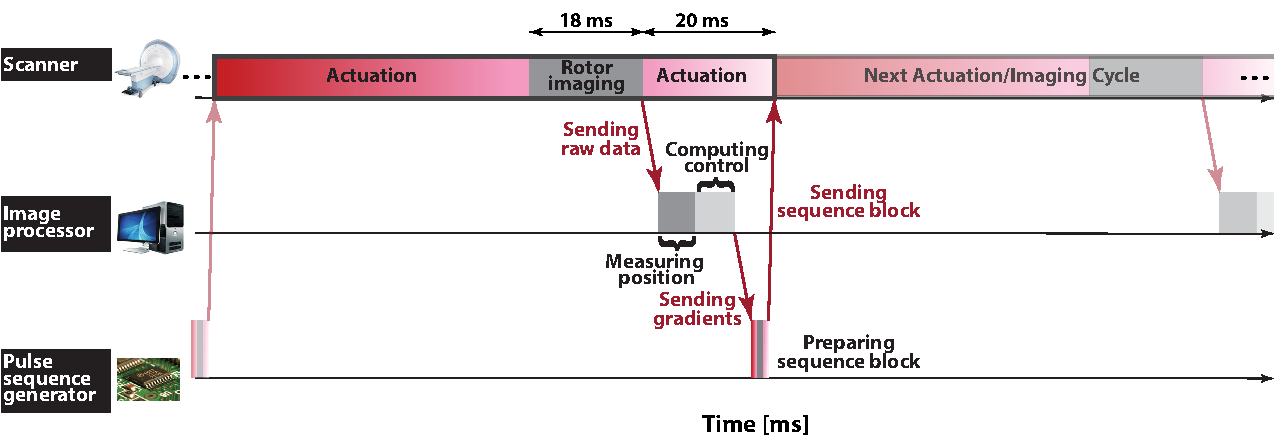
\includegraphics[width=1.89\columnwidth]{Figure5a.pdf}
		\label{fig:timing-diagram}
	}
	\subfigure[]{
		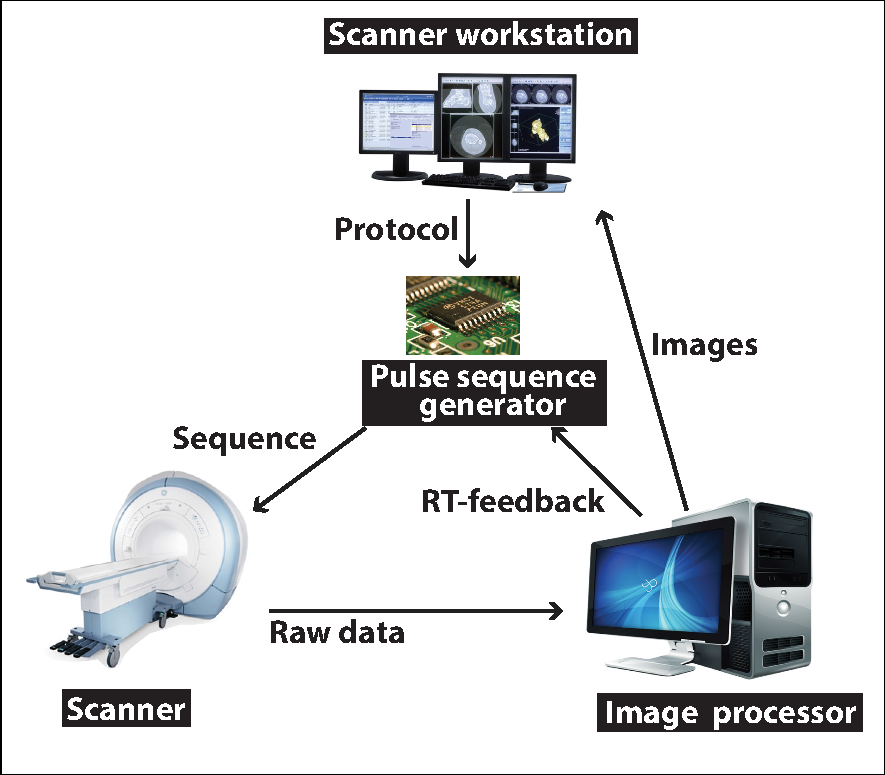
\includegraphics[width=0.73\columnwidth]{Figure5b.pdf}	
		\label{fig:control-architecture}
	}
	\subfigure[]{
		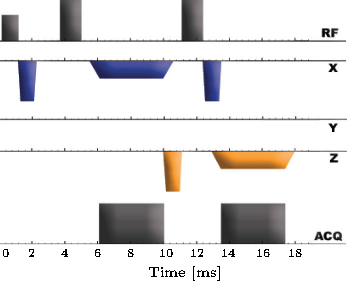
\includegraphics[width=0.8\columnwidth]{Figure5c.pdf}	
		\label{fig:Tracking-sequence}
	}
\end{center}
\caption{MRI architecture and pulse sequence design for closed-loop commutation. (a) Closed-loop pulse timing diagram, (b) Processor data flow diagram, and (c) Spin echo sequence to measure 1D projections of the rotor on the $x$ and $z$ axes.}
\vspace{-5pt}
\end{figure*}

After the tracking pulse sequence, the single-dimensional projections are transferred to the image processing workstation, where localization via peak detection is performed to measure the rotor position and imaging noise. As described below, a discrete-time state estimator uses this data to pre-compute the gradient directions for the two actuation components of the next pulse sequence. 


\section{Control and Estimation}
\label{sec:controlLaw}

A ferrous particle in the strong static field of an MRI scanner becomes magnetized, and its magnetization magnitude asymptotically approaches the saturation magnetization $\mathbf{M}_s$ per unit volume of the material.  The MRI gradient coils  produce a magnetic field  $\mathbf{B}_g(t)$. This field exerts 
 on the ferrous particle the force 
\begin{equation}
\mathbf{F}(t) = v\left( \mathbf{M}_s
\cdot \nabla \right) \mathbf{B}_g(t). \label{eq:forceOnDipole}
\end{equation}
Here $v$ is the magnetic volume of the material.  The magnetic field $\mathbf{B}_g(t)$ is designed to produce three independent gradients:
\begin{equation}
\left[ F_x,F_y, F_z \right]^\intercal\!\!(t)= v M_{sz}\left[  \frac{ \partial B_{gz}}{\partial x},  \frac{ \partial B_{gz}}{\partial y}, \frac{ \partial B_{gz}}{\partial z} \right]^\intercal\!\!\!\!(t)
\label{eq:applicableForces}
\end{equation}

Here it has been reasonably assumed that $M_{sz} \gg M_{sx}, M_{sy}$.
These three gradients apply three independent forces on any ferromagnetic sphere inside the MRI.  

The rotor construction constrains the ferromagnetic sphere to rotate about an axis $\mathbf{a}$ with a moment arm of length  $r$. Such a rotor is shown in Fig.~\ref{fig:actuator-illustration}.  The rotor's configuration at time $t$ is fully described by its angular position and velocity $[\theta(t), \dot{\theta}(t)]^\intercal$. Here $\theta$ is the angle referenced to the $x$-axis about the $y$-axis. The configuration space is $\R^{2}$,  and the dynamic equations are given by
\begin{equation}
\ddot{\theta}(t) = \frac{1}{J}\left(-b\dot{\theta}(t) -\tau_{f}-\tau_{\ell} + r \mathbf{F}(t)\cdot \mathbf{p}(t) \right)
\label{eq:rotorDynamics}
\end{equation}
Here $J$ is the moment of inertia, $b$ the coefficient of viscous friction,  $\tau_{f}$ the summation of all non-viscous friction terms seen by the input,  and $\tau_{\ell}$ the load torque. The rotor torque is the magnetic force projected  to a unit vector, $\mathbf{p}(t)$, tangent to the ferrous sphere's positive direction of motion, $r \mathbf{F}\cdot \mathbf{p}(t)$.  This model assumes that the rotor is perfectly balanced, and thus there is no gravity-related term. 

The goal of commutation control is to ensure that magnetic force is directed along $\mathbf{p}(t)$, such that $\mathbf{F}(t) = u(t) \mathbf{p}(t)$, where  $u(t)$ is a scalar control function. 

When the rotor axis is aligned with a coordinate axis, $\mathbf{p}(t)$ has a particularly simple form. The remainder of the paper will assume  $\mathbf{a} = \{0,1,0\}$. Given this choice,
\begin{align}
\ddot{\theta}(t) &= \frac{1}{J} \bigg( -b\dot{\theta}(t) -\tau_{f}-\tau_{\ell} +  \nonumber \\
& \qquad
 r \Big( F_z(t) \cos(\theta(t)) - F_x(t) \sin(\theta(t)) \Big)\bigg)
\label{eq:rotorDynamicsYAxis}
\end{align}
and the commutation control law is given by
\begin{align}
\begin{bmatrix}F_x\\F_y\\F_z\end{bmatrix} =  u(t)
\begin{bmatrix}
-\sin \theta(t) \\ 
0 \\ 
\cos \theta(t) \end{bmatrix}
\label{eq:ControlLaw}
\end{align}

Both the control and measurements are taken at discrete time intervals, so it is necessary to provide a discrete-time model.  This can be approximated by 
\begin{align}
\theta(k+1) &= \theta(k) + \dot{\theta}(k) T  \label{eq:rotorDynamicsDisc}\\
\dot{\theta}(k+1) &= \dot{\theta}(k) +  \frac{ T}{J}\left(-b\dot{\theta}(k) -\tau_{f}-\tau_{\ell} + r \mathbf{F}(k) \cdot \mathbf{p}(k) \right)  \nonumber
\end{align}
with time steps of  $T$ seconds.  

This model is used in combination with techniques for rotor angle measurement, state estimation and feedback control as described in the following subsections. 

\subsection{Rotor Angle Measurement}

The position of a stationary rotor can be measured using two orthogonal MRI line scans. 
The scans cannot be simultaneous. If the rotor is moving, these scans measure two 1D projections of the rotor's position at two different times, $t_1$ and $t_2$, where $t_2 = t_1 + \Delta T$:
\begin{align}
x(t_1) &= r \cos(\theta(t_1))  \nonumber \\
z(t_2) &= r \sin(\theta(t_2)), 
\label{eq:LineScanmeasurement}
\end{align}

To minimize movement between scans, a fast spin echo sequence shown in Fig. \ref{fig:Tracking-sequence} is used where the $x$ and $z$ scans are separated by $\Delta T = 7.5$ms. While the measured angle can be directly calculated as
\begin{equation}
\theta_M(t_2, \dot{\theta}) =\arctan\!\left( z(t_2), r\cos\! \left(\mathrm{arccos}(x(t_1)/r)+\dot{\theta} \Delta T \right) \right),
\label{eq:timefix}
\end{equation}
this equation uses the arccosine function, which is much less accurate using noisy data than computing the arctangent with both sine and cosine arguments. 

To avoid this inaccuracy, an alternate approach is introduced in terms of an intermediate measurement variable, $\theta_{M1}(t_1, t_2)$, which is computed using the arctangent function, 
\begin{align}
\theta_{M1}(t_1,t_2) = \arctan( z(t_2), x(t_1))
\label{eq:Anglemeasurement}
\end{align}
Assuming constant velocity, $\dot{\theta}_{12}$, over the interval $t\in\{t_1,t_2\}$, the error, $e$, between the desired measurement, $\theta_M (t_2)$, and the intermediate measurement variable, $\theta_{M1}(t_1,t_2)$, can be defined as a function of $\theta_{M1}(t_1,t_2)$ and $\dot{\theta}_{12}$,
\begin{align}
e(\theta_{M1}(t_1,t_2),\dot{\theta}_{12}) &= \theta_M(t_2,\dot{\theta}_{12}) - \theta_{M1}(t_1,t_2) 
\end{align}
and is plotted in Fig.~\ref{fig:RotorAngleErrorM1}. The error can be modeled by a Fourier series approximation in terms of $\theta_{M1}$ as
\begin{align}
e(\theta_{M1} , \dot{\theta}_{12}) \approx & \frac{a_0(\dot{\theta}_{12})}{2} + \sum_{n=1}^N a_n(\dot{\theta}_{12}) \cos(n \theta_{M1}) \nonumber \\
& + \sum_{n=1}^N b_n(\dot{\theta}_{12}) \sin(n \theta_{M1})
\end{align}
The Fourier series coefficients can be evaluated numerically using the standard integrals
\begin{align}
a_n(\dot{\theta}_{12}) & =  \frac{1}{\pi}\int_{-\pi}^{\pi} e(\alpha,\dot{\theta}_{12})\cos(n\alpha) \,\textrm{d}\alpha \nonumber\\
b_n(\dot{\theta}_{12}) & =  \frac{1}{\pi}\int_{-\pi}^{\pi} e(\alpha,\dot{\theta}_{12})\sin(n\alpha) \,\textrm{d}\alpha
\end{align}
At low velocities the approximation is dominated by $a_0$ and $a_2$, resulting in the 2$^{\text{nd}}$-order Fourier series approximation,
\begin{align}
\theta_M(t_2, \dot{\theta}) \approx \tilde{\theta}_M(t_2,  & \ \hat{\dot{\theta}}(t_2)) =  \theta_{M1}(t_1,t_2)  \nonumber \\
 +& \frac{\hat{\dot{\theta}}(t_2) \Delta T}{2}\Big(1-\cos(2\theta_{M1}(t_1,t_2))\Big) 
\label{eq:AnglemeasurementCorrected}
\end{align}
Here, the estimated velocity, $\hat{\dot{\theta}}(t_2)$, has been substituted for $\dot{\theta}_{12}$. Notice that the only inverse trigonometric evaluation in this approximation is the arctangent of \eqref{eq:Anglemeasurement}.

The correction terms of \eqref{eq:AnglemeasurementCorrected}, consisting of a zero frequency offset and a cosine of twice the rotor frequency are clearly visible in the error plot of Fig.~\ref{fig:Rotor-Angle-Corr}(a). The remaining error, depicted in Fig.~\ref{fig:Rotor-Angle-Corr}(b), is less than $2^\circ$ for angular velocities between $\pm10$ Hz. 

\begin{figure}
\begin{center}
	\subfigure[]{
		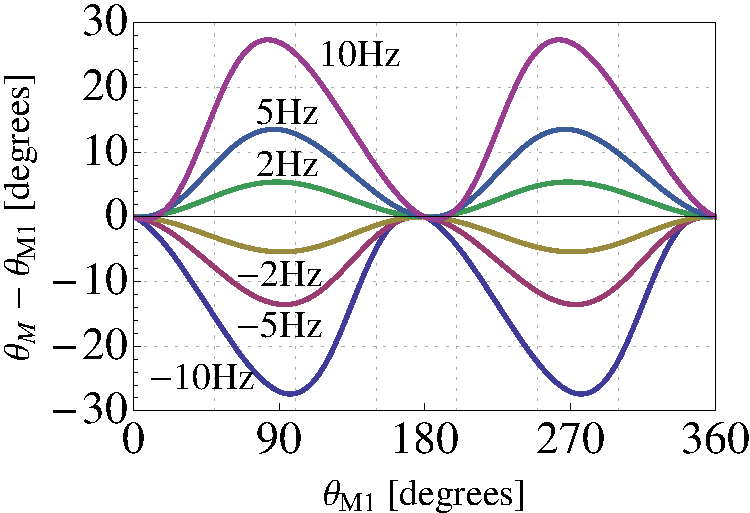
\includegraphics[width=0.48\columnwidth]{Figure6a.pdf}
		\label{fig:RotorAngleErrorM1}
	}\subfigure[]{
		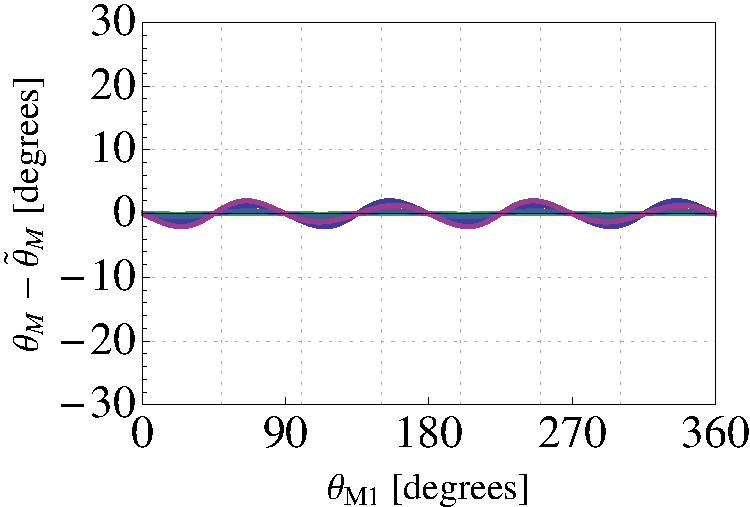
\includegraphics[width=0.48\columnwidth]{Figure6b.pdf}
		\label{fig:RotorAngleErrorM}
	}
\end{center}
\caption{Rotor angle error due to time delay of $\Delta T = 7.5$ms between axial projections. (a) Error when time delay is ignored using \eqref{eq:Anglemeasurement}. Negative frequencies correspond to negative rotational velocities. (b) Error using corrected angle estimate, $\theta_M$, from \eqref{eq:AnglemeasurementCorrected}. 
\label{fig:Rotor-Angle-Corr}}
\end{figure}


\subsection{State Estimator}
The rotor position can be measured several times per second, but the control law (Sec.\ \ref{subsec:ExpMaxTorque}) requires the position and velocity several hundred times per second.
To provide state estimates between measurements as well as to compensate for imaging noise, Kalman filtering is employed. The state equations at step $k$ are linearized about the estimated state given all sensor measurements at time $k$: $[\hat{\theta}(k|k),\hat{\dot{\theta}}(k|k) ]$. Following the standard approach, estimation is split into \emph{predicting} the current state using previous measurements and the process model and  \emph{correcting} the estimate using MRI measurements. State estimates, $\hat{\theta}$ and $\hat{\dot{\theta}}$, and estimate covariances, $P_{\theta}$ and $P_{\dot{\theta}}$, are predicted using
\begin{align}
\hat{\theta}(k+1|k) &= \hat{\theta}(k|k) + T \hat{\dot{\theta}}(k|k) \nonumber \\
\hat{\dot{\theta}}(k+1|k) &= \hat{\dot{\theta}}(k|k) +  \frac{T}{J}\bigg(-b\hat{\dot{\theta}}(k|k)  -\tau_{f}-\tau_{\ell}  \nonumber \\
&  + r \left( F_z(t) \cos(\hat{\theta}(k|k) ) - F_x(t) \sin(\hat{\theta}(k|k) ) \right)\bigg) \nonumber \\
P_{\theta}(k+1|k) &= P_{\theta}(k|k)  + Q_{\theta}\nonumber \\
P_{\dot{\theta}}(k+1|k) &= P_{\dot{\theta}}(k|k)  + Q_{\dot{\theta}}
\label{eq:StateUpdate}
\end{align}

The state estimates and covariances are corrected as follows
\begin{align}
\hat{\theta}(k+1|k+1) &= \hat{\theta}(k+1|k) \nonumber \\
& \left. + K_{\theta}(k+1)\Big(\theta_M(k+1) -\hat{\theta}(k+1|k)\Big)  \right.\nonumber \\
\hat{\dot{\theta}}(k+1|k+1) &= \hat{\dot{\theta}}(k+1|k) \nonumber \\
& \left. +  K_{\dot{\theta}}(k+1)\Big(\dot{\theta}_M(k+1) -\hat{\dot{\theta}}(k+1|k)\Big)  \right.\nonumber \\
P_{\theta}(k+1|k+1) &= \Big( 1 -  K_{\theta}(k+1)    \Big)P_{\theta}(k+1|k)   \nonumber\\
P_{\dot{\theta}}(k+1|k+1) &= \Big( 1 -  K_{\dot{\theta}}(k+1)    \Big)P_{\dot{\theta}}(k+1|k)  
\label{eq:StateCorrection}
\end{align}

The correction uses MRI measurements of the rotor orientation $\theta_M(k+1)$ and a finite difference calculation of the rotor angular velocity $\hat{\dot{\theta}}_M(k+1)$, along with the measurement noise $R_{\theta}(k+1)$ and $R_{\dot{\theta}}(k+1)$. Measurement noise is calculated using a statistical property of the MRI scan quality, as described in Sections \ref{subsec:CNR} and \ref{subsec:ExpNoiseProperties}.
The optimal Kalman gains $K_{\theta}(k+1)$ and $K_{\dot{\theta}}(k+1)$ are calculated as
\begin{align}
K_{\theta}(k+1) &= P_{\theta}(k+1|k) ( P_{\theta}(k+1|k)  + R_{\theta}(k+1))^{-1} \nonumber \\
K_{\dot{\theta}}(k+1) &= P_{\dot{\theta}}(k+1|k) ( P_{\dot{\theta}}(k+1|k)  + R_{\dot{\theta}}(k+1))^{-1} 
\label{eq:StateCorrectionKalmanGain}
\end{align}
Performance of the state estimator is described in Section \ref{subsec:ExpNoiseProperties}.

\section{Experiments}
\label{sec:experiments}
To evaluate the tracking and commutation control methods described above, a series of analyses and experiments were performed. The subsection below describes the optimization of fiducial marker location as well as the imaging parameters used to image rotor angle. Since MR imaging has not been previously applied to rapidly moving objects,  a series of experiments described in Section \ref{subsec:CNR} investigate how image quality varies with sampling rate and rotor velocity. Evaluation of the state estimator is described in Section \ref{subsec:ExpNoiseProperties}. Experimental validation of two types of closed-loop commutation controllers is also presented in Sections \ref{subsec:ExpMaxTorque} and \ref{subsec:ExpClosedLoopPositionControl}. A maximum torque controller is used to compare the stall torque that can be achieved in closed- versus open-loop commutation. Finally, it is demonstrated how closed-loop commutation enables control of rotor position.

All experiments used the prototype actuator shown in Fig.\ \ref{fig:experimental-setup}. The system consists of a rotor driving a gear train attached to a rack. While prior work used a rack-mounted needle to perform tissue insertion experiments \cite{bergeles2012tracking}, a needle was not used here and, for some tests, a set of calibrated springs was attached as shown to generate a linearly increasing load. The prototype is constructed from LEGO\texttrademark~Technic blocks. It is MRI-invisible and compatible. Prototype parameters are given in Table\ \ref{tab:parameters}. 
Friction and inertia parameters were estimated through calibration experiments.
Imaging parameters are given in Table\ \ref{tab:imagingparameters}. 
Real-time communication was achieved using the Siemens Integrated Development Environment for Applications (IDEA). A Canon single-lens reflex video camera (model T1i) was used to record rotor position for ground truth measurements by mounting an angled mirror behind the prototype, and placing the camera on a tripod outside the 5-Gauss line. Color thresholding was used to detect a red marker mounted on the rotor arm. Each video frame was transformed to a binary image showing the red marker as white and the background as black.  The center of mass of these white pixels was used to find the rotor location. The spatial resolution of the video camera was $\sim$0.2mm, $\sim$3x the MRI resolution. The frame rate of the video camera was also superior to the MRI acquisition rate with 30 frames per second, an increase of two to three times the MRI imaging rate.

\begin{table}[b]
\vspace{-10pt}
\centering
\scriptsize
\caption{Prototype Actuator Parameters}
\label{tab:parameters}
\begin{tabular}{r | c}
	\textbf{Parameter}  & \textbf{Value} \\
	\hline
	Radius of ferrous sphere & $5\,$mm \\
	Saturation magnetization of ferrous sphere & $1.36\times10^6\,$A/m \\
	Rotor arm radius $r$& $32.5\,$mm \\
	Transmission ratio & $125$ \\
	Fiducial marker radius & $3.5\,$mm \\
	Fiducial marker height & $16\,$mm \\
	Fiducial marker offsets $r_d$, $\textnormal{v}_d$ & $ \sim0.0\,$mm, $\sim87\,$mm 
\end{tabular}
\normalsize
\end{table}


\begin{table}[b]
\vspace{-10pt}
\centering
\scriptsize
\caption{Imaging Parameters}
\label{tab:imagingparameters}
\begin{tabular}{r | c}
	\textbf{Parameter}  & \textbf{Value} \\
	\hline
	Static magnetic field $\norm{\vec{B}_0}$ & $3\,$T\\
	Echo time $x$, $\textnormal{TE}_{x}$ & $7.5\,$ms\\
	Echo time $z$, $\textnormal{TE}_{z}$ & $15\,$ms\\ 
	Field of view ($\textnormal{FOV}$) & $300\,$mm\\
	Flip angle  $\alpha$ & $90^\circ$\\
	$\textnormal{Matrix}$ & $512\,$pixels\\
	$\textnormal{RF-offset}$ & $-3500\,$Hz\\
	Spatial resolution & $0.59\,$mm  \\
	The tracking pulse sequence $t_\textnormal{track}$&$ 18\,$ms
\end{tabular}
\normalsize
\end{table}



\begin{figure}[t]
\begin{center}
	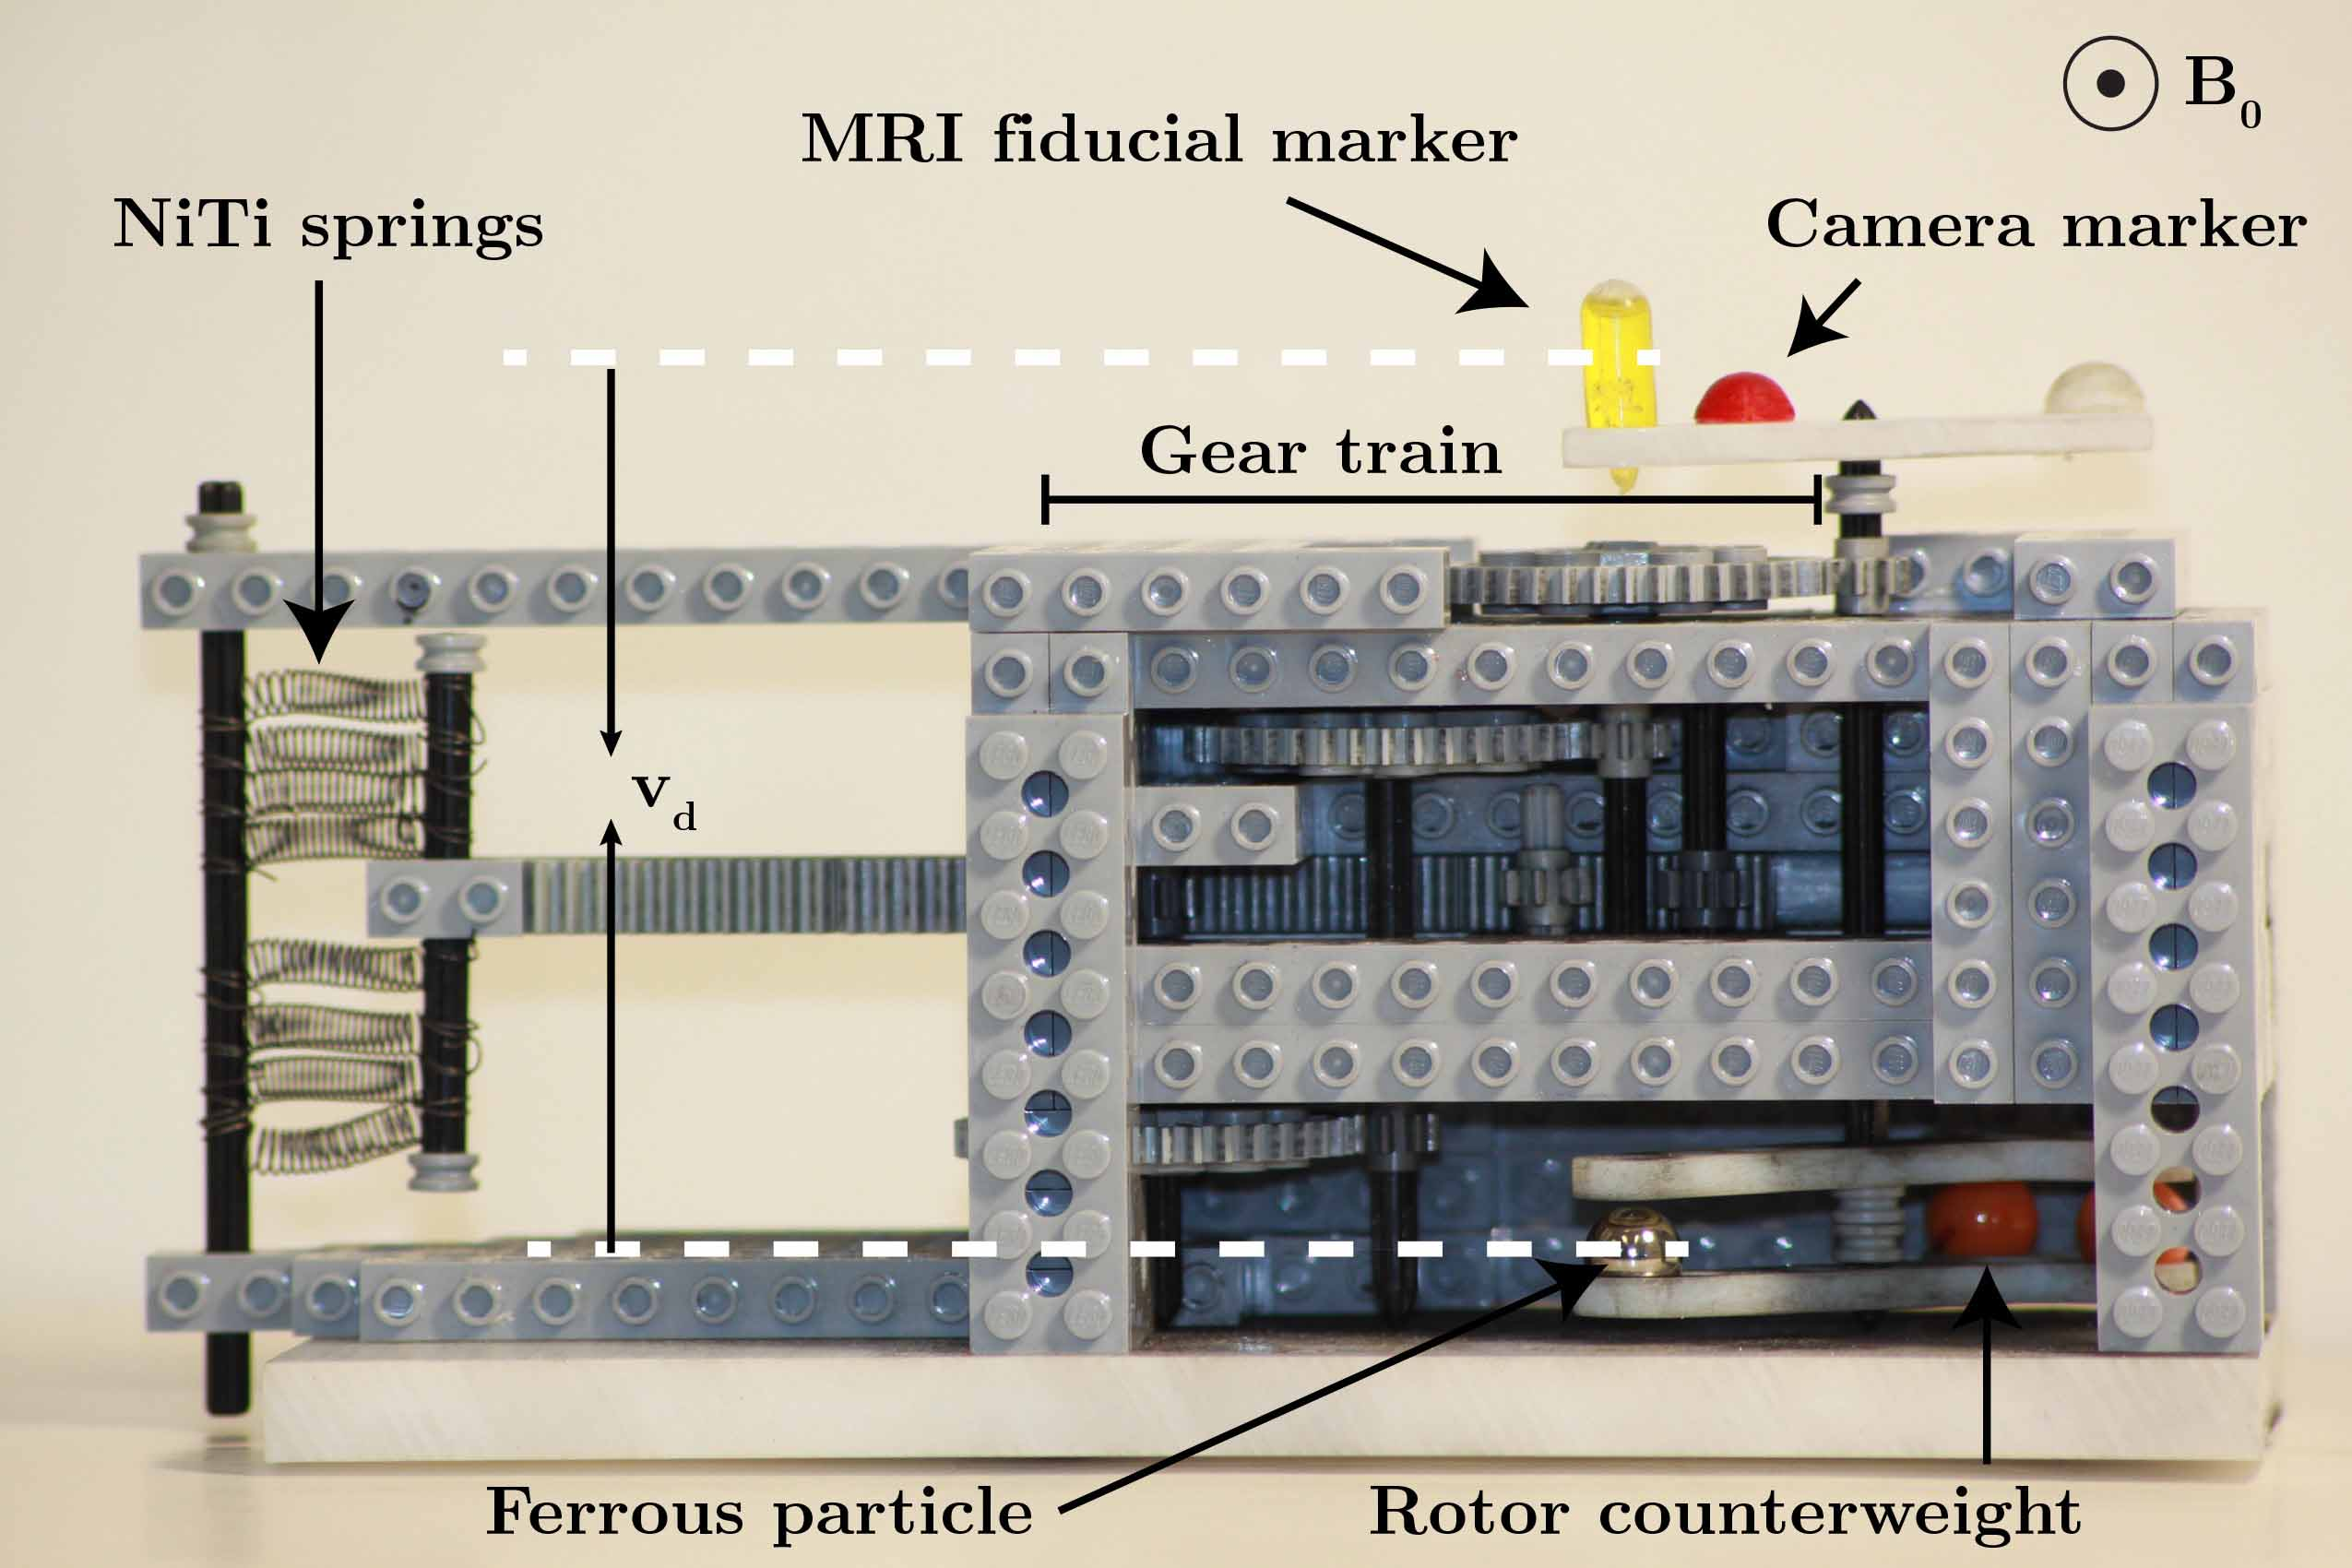
\includegraphics[width=0.9\columnwidth]{Figure7.jpg}
\end{center}
\caption{Actuator used in experiments.}
\label{fig:experimental-setup}
\vspace{-10pt}
\end{figure}

\subsection{Optimizing Fiducial Location and Imaging Parameters}\label{subsec:rotorImaging}

\begin{figure}
\begin{center}
	\subfigure[]{
		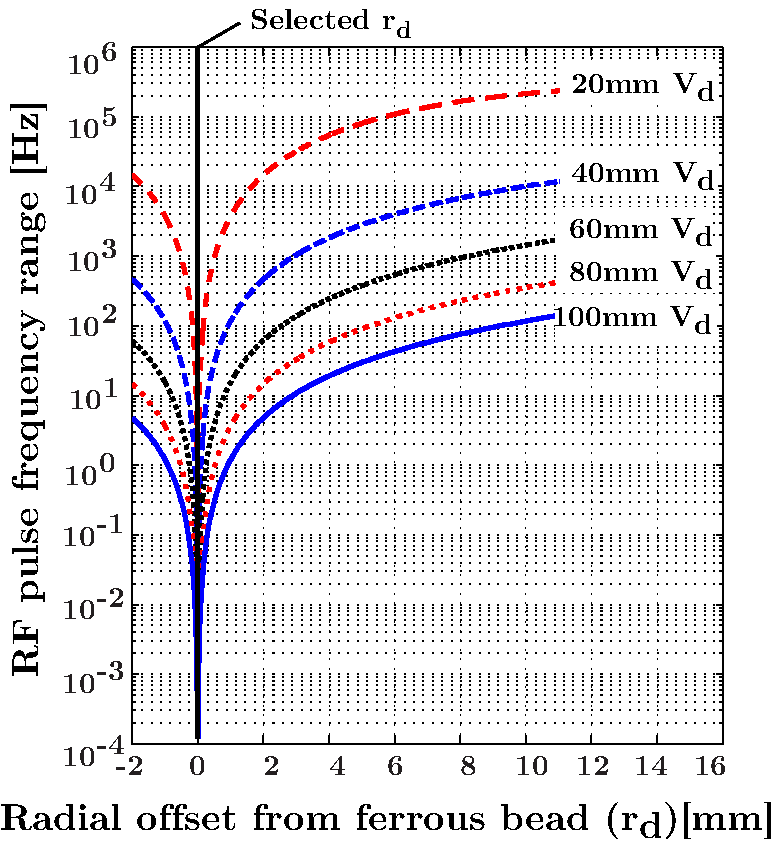
\includegraphics[width=0.43\columnwidth]{Figure8a.pdf}
		\label{fig:rotation-dependent-rf}
	}
	\subfigure[]{
		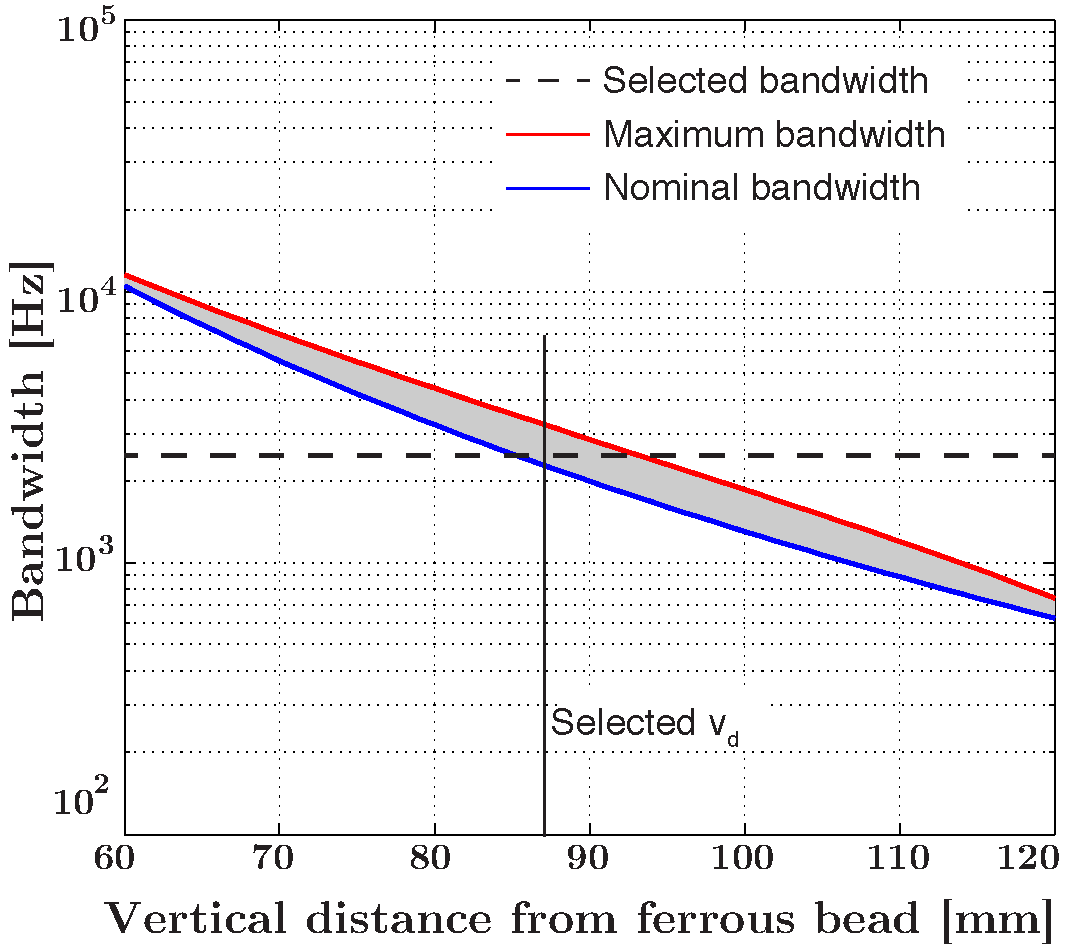
\includegraphics[width=0.50\columnwidth]{Figure8b.pdf}		
		\label{fig:bandwidth-with-respect-to-distance}
	}		
\end{center}
\caption{Selection of marker location. (a) Dependency of the RF pulse on $r_d$ for different values of  $\textnormal{v}_d$. (b) Dependency of the RF bandwidth on $\textnormal{v}_d$. Dashed line represents the bandwidth corresponding to a $1\,$ms duration RF. For the selected bandwidth, vertical distances between  $85\le \textnormal{v}_d \le 94\,$mm constitute a nominal combination that covers the entire marker without causing any background excitation.}
\vspace{-10pt}
\end{figure}

\begin{figure}[t]
\begin{center}
	\subfigure[]{
		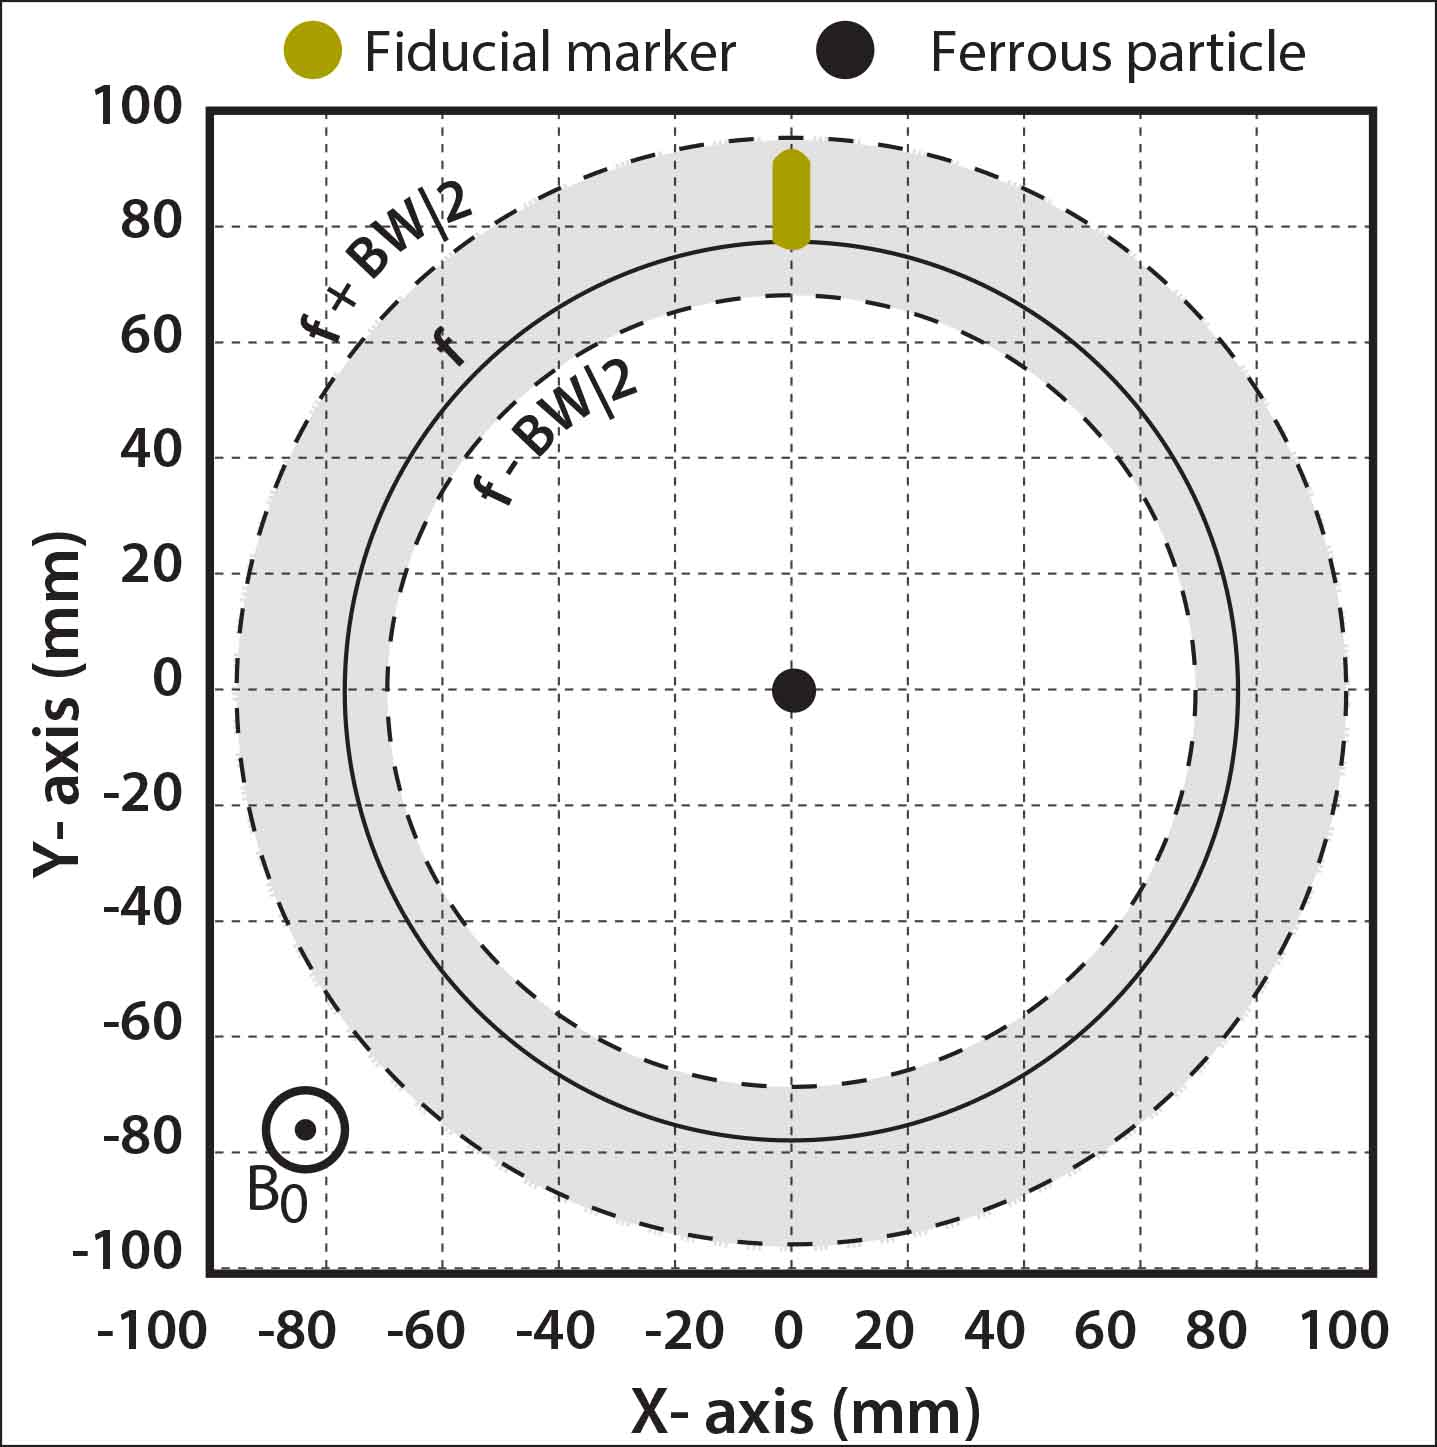
\includegraphics[width=0.42\columnwidth]{Figure9a.jpg}
	}
	\subfigure[]{
		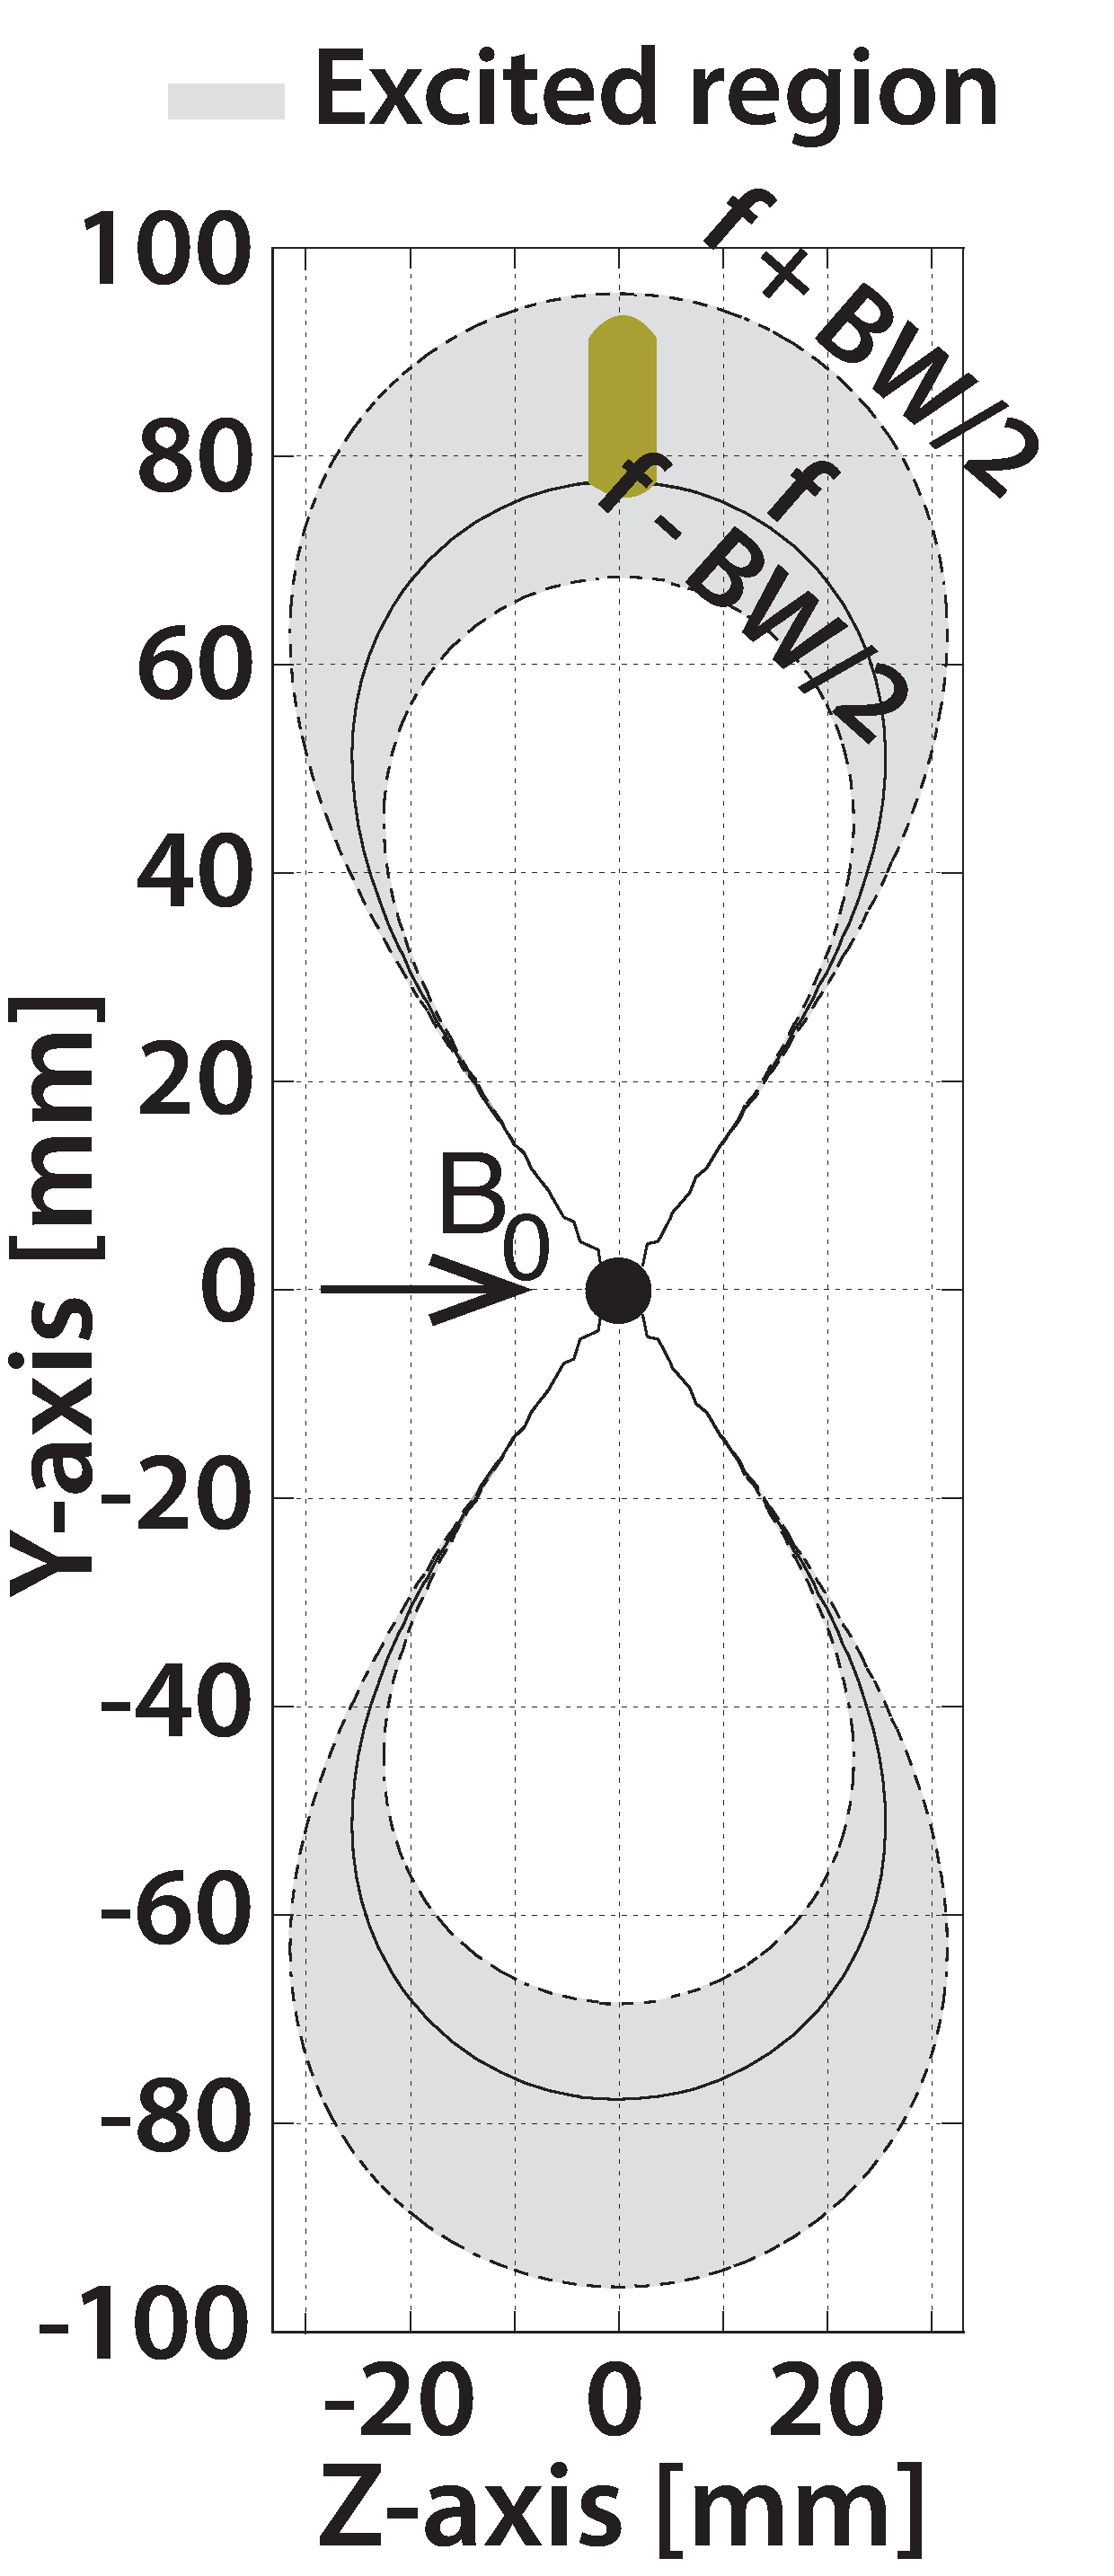
\includegraphics[width=0.189\columnwidth]{Figure9b.pdf}
	}
	\subfigure[]{
		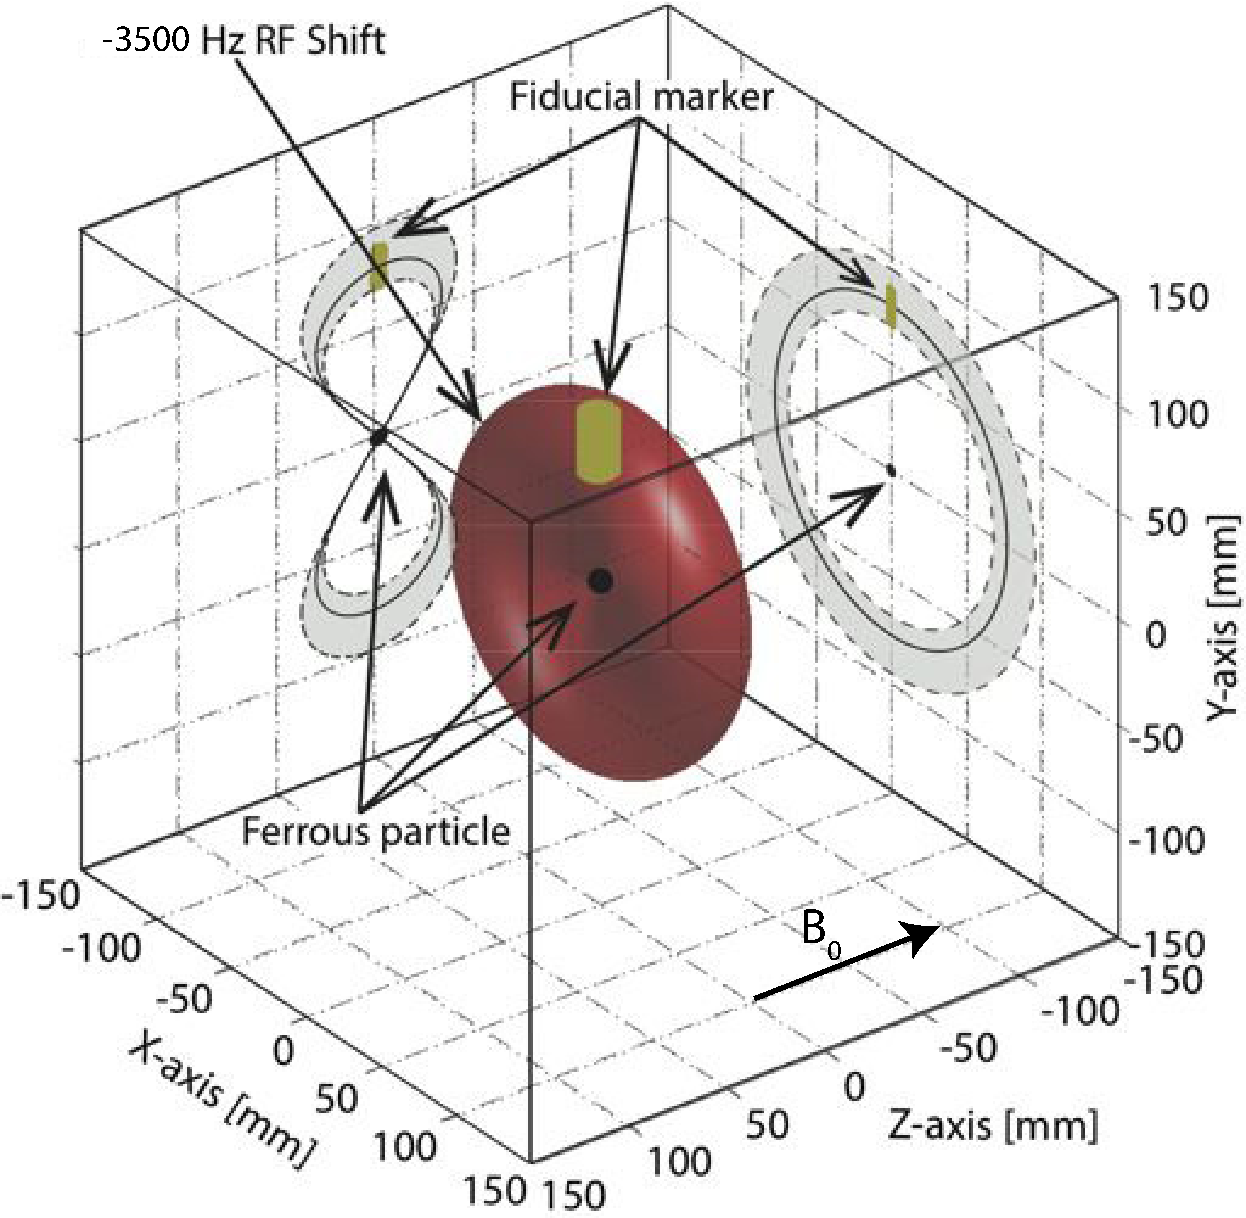
\includegraphics[width=0.6\columnwidth]{Figure9c.pdf}
	}
\end{center}
\caption{Region of RF-selected excitation. (a) XY plane, (b) ZY plane, (c) 3D view with projections. Solid lines indicate surface excited at central RF frequency; dashed lines indicate volume excited over bandwidth.}
\label{fig:fiducial-in-field}
\vspace{-10pt}
\end{figure}

An \href{http://www.beekley.com/MRI/MRSPOTS.asp}{MR-SPOT (Beekley Medical, CT)} marker's location was optimized for imaging the ferrous particle contained within the actuator, as described in Sec.\ \ref{sec:tracking}. Fig.\ \ref{fig:rotation-dependent-rf} shows the range of frequencies required for various displacements $r_d$. This simulation shows that to measure rotor angle using an RF pulse with constant central frequency and varying rotor angles, there should be no radial displacement of the fiducial marker with respect to the ferrous particle, i.e. $r_d = 0\,$mm.
 
The required RF-pulse bandwidth with respect to the vertical distance $\textnormal{v}_d$ is shown in Fig.\ \ref{fig:bandwidth-with-respect-to-distance}. The dashed line corresponds to the bandwidth of a $1\,$ms RF pulse ($2.5\,$kHz), the nominal pulse width. For this pulse width the optimal vertical offset to excite the full marker volume without causing background excitation is $85\le \textnormal{v}_d \le 94\,$mm (see Fig.\ \ref{fig:fiducial-in-field}).

These selections of $r_d$ and $\textnormal{v}_d$ define $ \vec{P}_m(r_d,\textnormal{v}_d)$ and (\ref{eq:dipole-model})-(\ref{eq:frequency}) can now be used to solve for an RF-offset of $ -3.5\,$kHz. Given the choice of $\textnormal{BW} = 2.5\,$kHz in the paragraph above, it can be verified that these values satisfy \eqref{eq:below} ensuring that no signal emission from tissue will arise during fiducial tracking. The resulting volume of excitation around the ferrous sphere is depicted in Fig. \ref{fig:fiducial-in-field}. The capsule-shaped fiducial marker is entirely within the excited region. Moreover, its excitation is independent of rotor angle. 


\subsection{Image Quality} \label{subsec:CNR}


Imaging was performed using a 32-channel head coil. Because the signal emitted from the marker is not evenly detected by all the channels, the weighted average $\bar{S}$ was used:
 \begin{equation}
	\bar{S} = \sqrt{\sum_{i=1}^{32} cnr_i S_i^{2}}
\label{eq:CombinedSignal}
\end{equation}
where $S_i$ is the signal detected by the $i^{th}$ channel and $cnr_i$ is the \emph{Contrast-to-Noise Ratio} of the $i^{th}$ channel given by:

\begin{align}
    cnr_i &= \dfrac{CNR_i}{\sum_{j=1}^{32} CNR_j} \nonumber\\
    CNR &= \dfrac{\abs{S_{A}-S_{B}}}{\sigma_{\circ B}}
\label{eq:CNR}
\end{align}
where $S_{A}$ is the maximum value measured in a region containing possible marker positions (depicted by the rectangular window shown in \ref{fig:CNR}), $S_{B}$ is the maximum value measured in a region of interest outside the rotor arm revolution, and $\sigma_{\circ B}$ is the standard deviation measured in the same region of interest outside the rotor arm revolution. Higher CNR values correspond to higher peak detection accuracy. CNR was used to assess the effects on imaging of nearby tissue as well as sampling rate and rotor velocity as described below.

\subsubsection{Effect of nearby tissue}\label{subsubsec:ExpNonwMovingTrackingWithPhantom}
The goal of RF-selective excitation is to create a strong signal from the fiducial marker for tracking the rotor while avoiding excitation of nearby tissue. This is necessary since the tissue signal would make it difficult to pick out the peak corresponding to the rotor in the $x$- and $z$-axis projections. To examine this issue, experiments were conducted with and without a 5.3L liquid-filled cylindrical container (Siemens MR Phantom) that was placed on the rack side of the actuator to simulate tissue located appropriately for needle biopsy.

Tracking accuracy for a stationary rotor was evaluated for angles between $0^\circ$ and $360^\circ$ in $15^\circ$ steps using a 24-position jig. The scanner's laser positioning system was used to position and orient the rotor at the scanner's isocenter. For each rotor angular position, 20 measurements at a 10Hz rate were acquired. Peak detection was performed only inside the possible spatial range of the rotor and no filtering was used. To correct for registration errors associated with laser-assisted manual fixture placement, the data acquired without the water-filled phantom were used to estimate the rotor center in the plane as well as the rotation of the fixture about the vertical axis. These calibration values were then used to compute angle error with and without the water-filled phantom. 

Results are shown in Fig.\ \ref{fig:localization-results}. Measurement error without the tissue phantom is zero mean (as a result of registration) with a standard deviation of $\pm1.65^\circ$. With the tissue phantom in place, the mean error is $0.35^\circ \pm 1.53^\circ$. Thus, the placement of tissue adjacent to the actuator has negligible effect on rotor imaging. 

\begin{figure}
			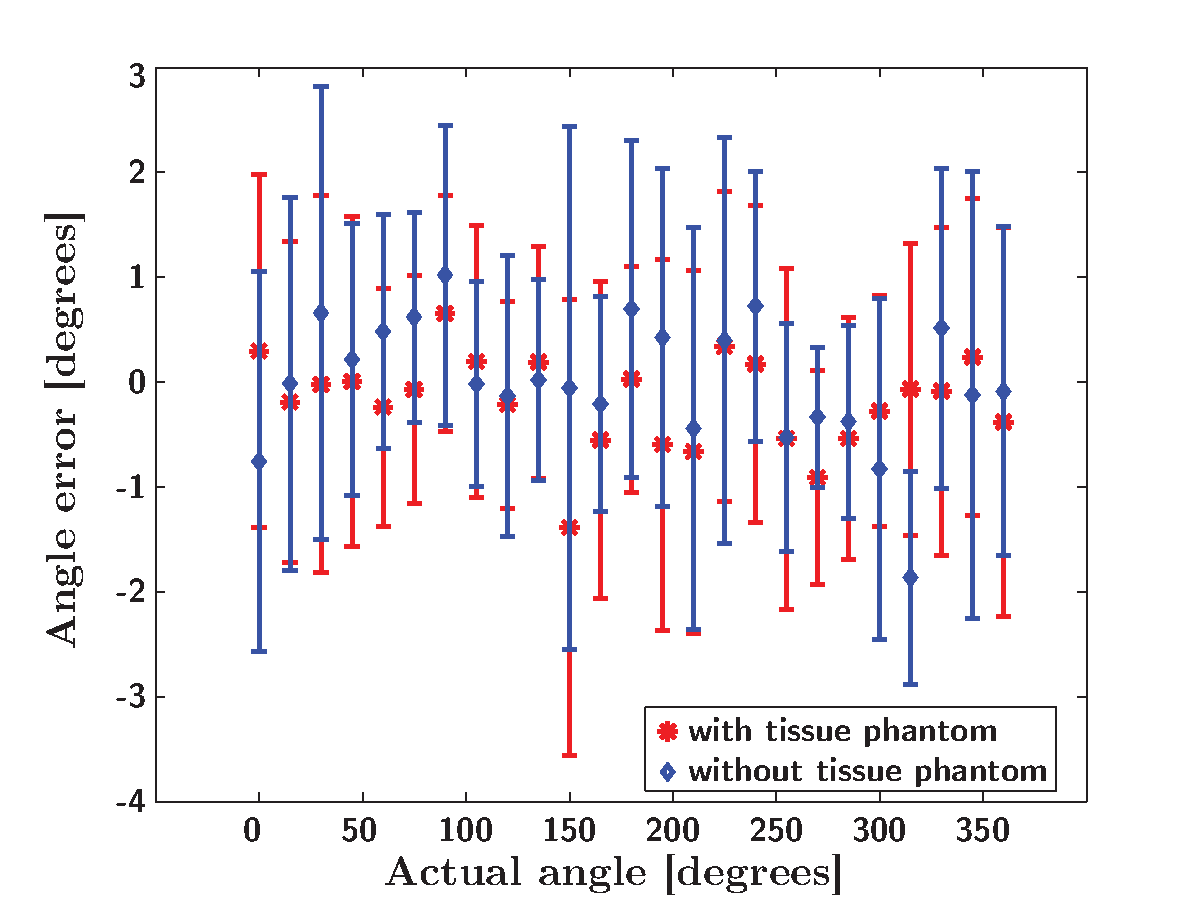
\includegraphics[width=1.0\columnwidth]{Figure10.pdf}
		
\caption{Image-based angle error measurement for a stationary rotor. Blue $\Diamond$: angle error without water-filled tissue phantom, Red *: angle error in the presence of water-filled tissue phantom. \label{fig:localization-results} }

\end{figure}

\begin{figure}
		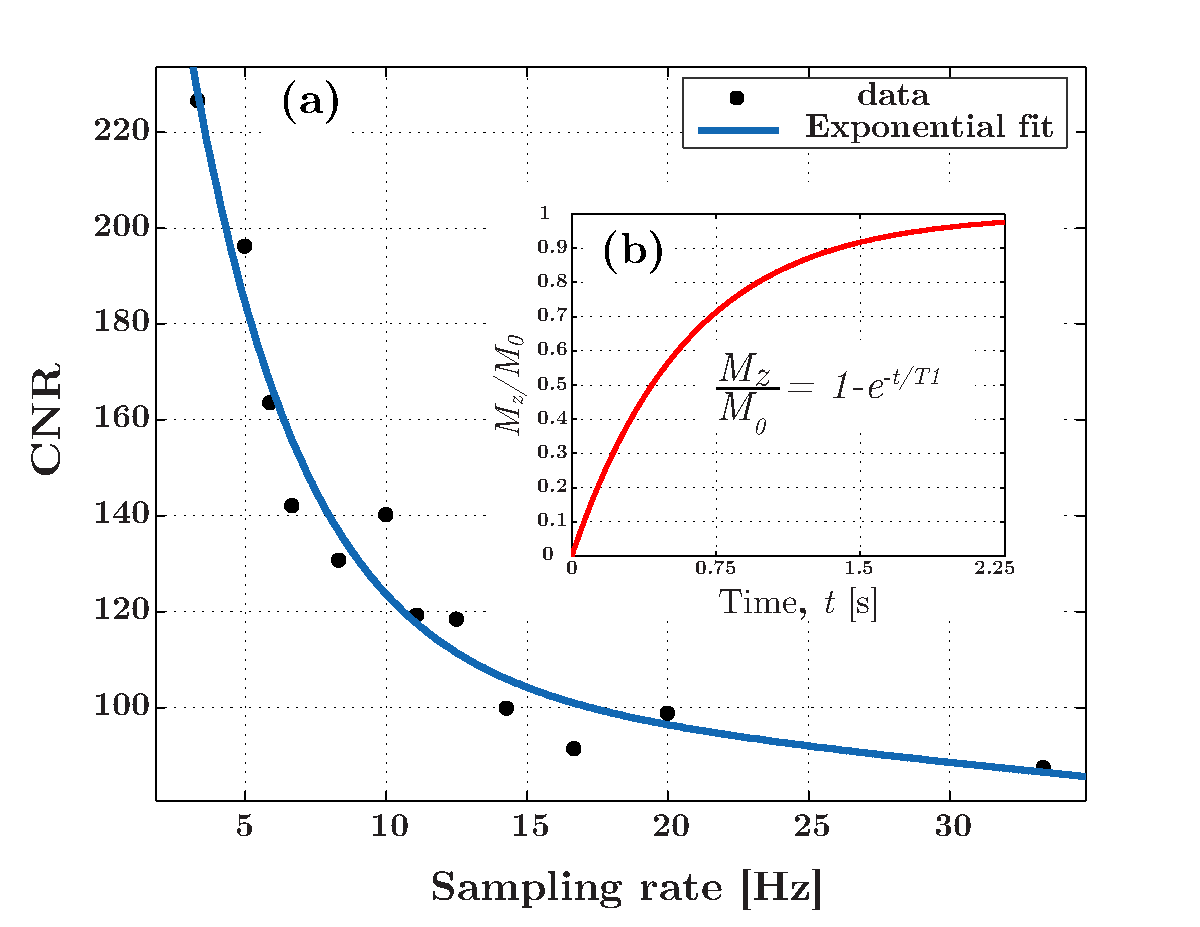
\includegraphics[width=1.0\columnwidth]{Figure11.pdf}

\caption{Effect of sampling rate on image quality. (a) Steady-state contrast-to-noise ratio (CNR) as a function of sampling rate for a stationary rotor. (b) $T_1$ relaxation curve showing regrowth of longitudinal component of magnetization from the initial value $M_z = 0$ following the excitation to the equilibrium value $M_0$ for an MRI fiducial with $T_1 = 540$ms.}
\label{fig:CNR-Vs-SamplingRate}

\end{figure}

\subsubsection{Effect of Sampling Rate on Imaging}\label{subsubsec:ExpImagingSamplingRate}
The time between two consecutive imaging cycles affects the signal intensity based on $T_1$, the longitudinal relaxation time of the marker. This quantity is the decay constant for the regrowth of the $z$ component of the magnetization, $M_z$. When the sampling rate is high, the $M_z$ available for the next excitation is small, as described by the regrowth plot in Fig.\ \ref{fig:CNR-Vs-SamplingRate}b. Decreasing the time between images decreases the signal strength. 
Fig.\ \ref{fig:CNR-Vs-SamplingRate} depicts this effect for a stationary rotor, showing that CNR decreases exponentially with increasing sampling rate.

\subsubsection{ Effect of Rotor Angular Velocity on Imaging}
\label{subsubsec:ExpImagingAngVelocity}
Motion artifacts are known to cause blurring and ghosting in MR images. Similarly, rotor motion during marker imaging can be anticipated to decrease the peak amplitude of the marker projections. To investigate this effect, CNR was computed and plotted along with rotor velocity as shown in Fig.\ \ref{fig:CNR-Vs-AngularVelocity}. It can be observed that CNR is inversely related to rotor angular velocity. Figure \ref{fig:CNR} provides examples of MRI projections for three different angular velocities illustrating how the signal peak can reduce to that of the background noise level as velocity increases. Note that for the highest velocities depicted in this figure, it is still possible to track the rotor since (1) not all projections taken at high velocity exhibit the weak amplitude depicted in the rightmost plot, (2) the peak search is restricted to the rotor arm distance, a region in which the highest peak much of the time corresponds to the marker position. In addition, the CNR value is tracked and used by a state estimator to update the rotor location as presented in Section \ref{subsec:ExpNoiseProperties}.


\begin{figure}
\begin{center}
\subfigure[CNR during calibration and commutation control]{
		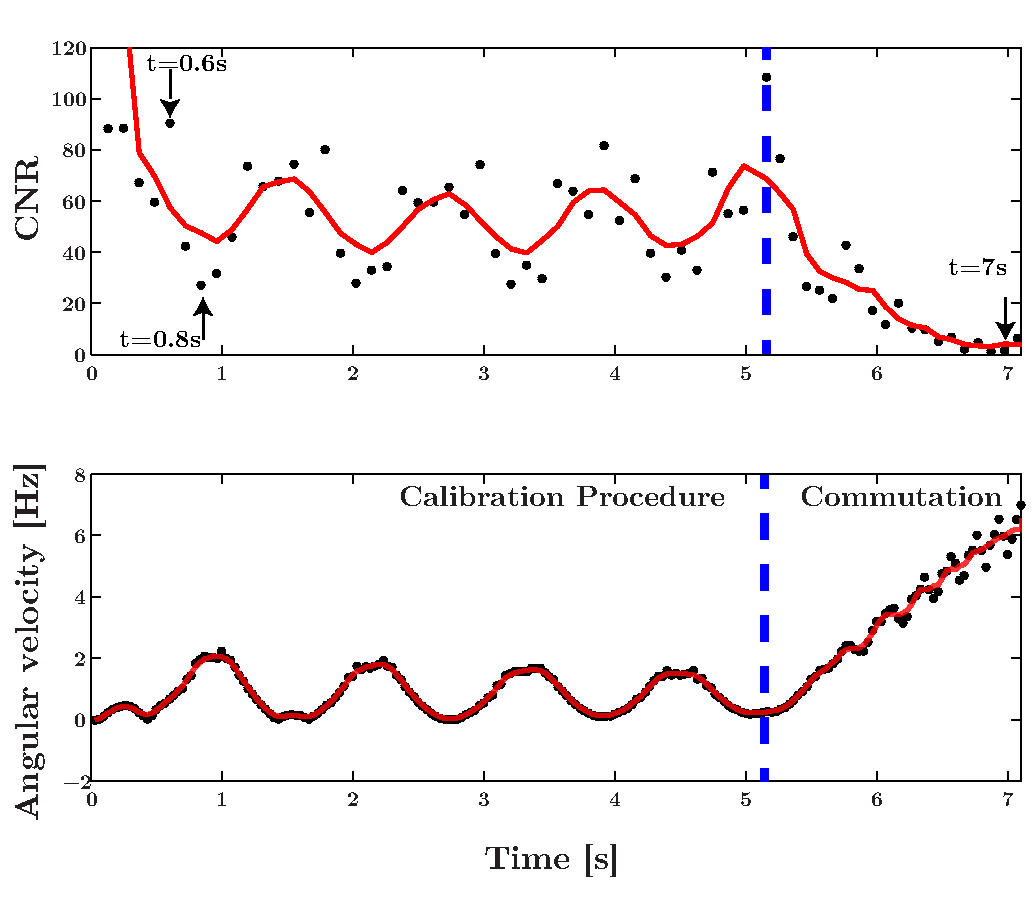
\includegraphics[width=0.8\columnwidth]{Figure12a.pdf}
		\label{fig:CNR-Vs-AngularVelocity}
		}
	\subfigure[MRI projections for three rotor velocities]{
		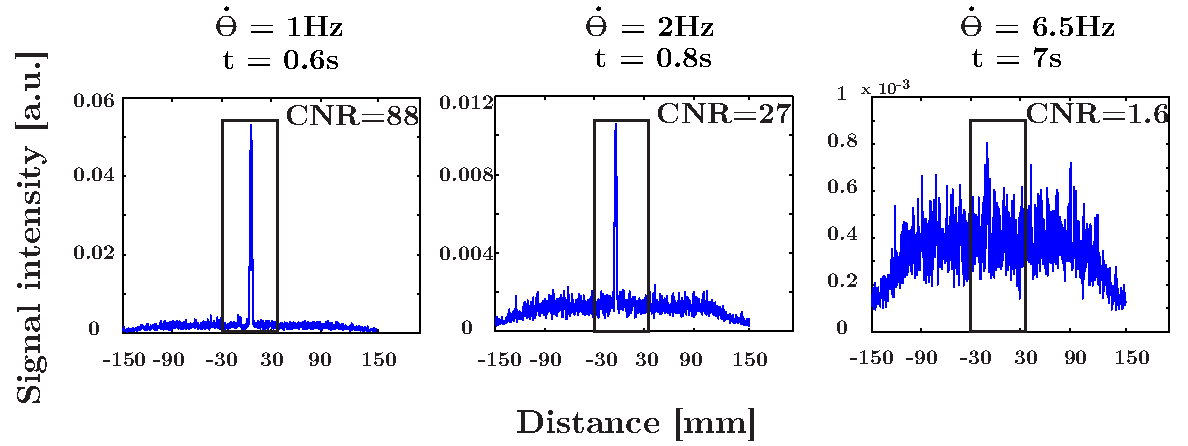
\includegraphics[width=1\columnwidth]{Figure12b.pdf}
		\label{fig:CNR}
		}
\end{center}
\caption{Relationship between CNR and rotor velocity, $\dot{\theta}$. (a) Example plot showing initial rotor calibration with oscillating rotor velocity followed by closed-loop commutation during which velocity increases. (b) Projections for three times from (a) corresponding to different velocities. The rectangular windows denote the possible marker positions used for calculating CNR. They are calculated from rotor arm center location and radius. Note how CNR decreases with increasing rotor velocity. }
\end{figure}


\subsection{State Estimation}\label{subsec:ExpNoiseProperties}
While it is assumed here that the actuator rotates about the $y$-axis, the location of its center of rotation inside the scanner bore is arbitrary. Consequently, a calibration pulse sequence was developed to estimate the point corresponding to the center of rotation of the fiducial marker. This open-loop sequence interleaves gradients rotating in the $xz$ plane with imaging sequences to detect and track the marker. 
The center of rotation is estimated by fitting a circle to the set of marker data points \cite{Pratt:1987:DLF:37402.37420}. Once the center of rotation is estimated, closed-loop commutation control begins automatically. The calibration and transition to closed-loop control are illustrated in the data set of Fig.~\ref{fig:CNR-Vs-AngularVelocity}.  

Rotor angle is computed from line scans along the $x$ and $z$ axes using (\ref{eq:Anglemeasurement})-(\ref{eq:AnglemeasurementCorrected}). The state estimate is then corrected according to \eqref{eq:StateCorrection}   with measurement noise given by 

\begin{align}
%\begin{equation}
%R_{\theta}(k+1) = 0.0012 \hat{R}
%R_{\theta}(k+1) =  0.0012 + \frac{10}{min(10,CNR)}-1 
	R_{\theta}(k+1) &= \hat{R} + \frac{10}{min(10,CNR)}-1, \nonumber \\
	R_{\dot{\theta}}(k+1) &= \Delta T^{-2}\bigg( R_{\theta}(k+1) + R_{\theta}(k)\bigg),
\label{eq:MeasurementNoise}
\end{align}

where $\hat{R}$ is the measurement noise due to discretization and  $CNR$ is the contrast-to-noise ratio calculated for the combined channels in \eqref{eq:CNR}. The cutoff $CNR \geq 10$ is heuristically determined because projection data with large $CNR$ have an easily distinguishable peak corresponding to the marker. For $CNR<10$ the peak can be indistinguishable from the background noise. Since the rotor velocity is computed using a first-order finite difference method, the measurement velocity noise, $R_{\dot{\theta}}$, is given by the linear combination of two independent variables.

The performance of the estimator during closed-loop commutation is illustrated in Figure \ref{fig:Estimate-Performance-PlusZoom}. This figure plots estimated rotor angle, MRI-based measurements of rotor angle, and estimated covariance of rotor angle. In addition, rotor angle as measured by the video camera is also plotted. Gaps in estimated rotor angle correspond to the 18ms intervals during which MRI imaging occurs and actuation is suspended. 

Computation of image processing, estimation and control together with pulse sequence generation require an additional 20ms before the state estimate used for actuation can be updated to include the latest rotor angle measurement. Consequently, the depicted covariance decreases 20ms after completion of each imaging sequence at the instant when the updated state estimate (denoted with a blue `*') becomes available. Comparison of estimated angle with video camera measurements reveals accurate tracking of actual rotor angle.  The absolute tracking error, averaged over all trials, was 4.42$^\circ$.  

\begin{figure}
\begin{center}
	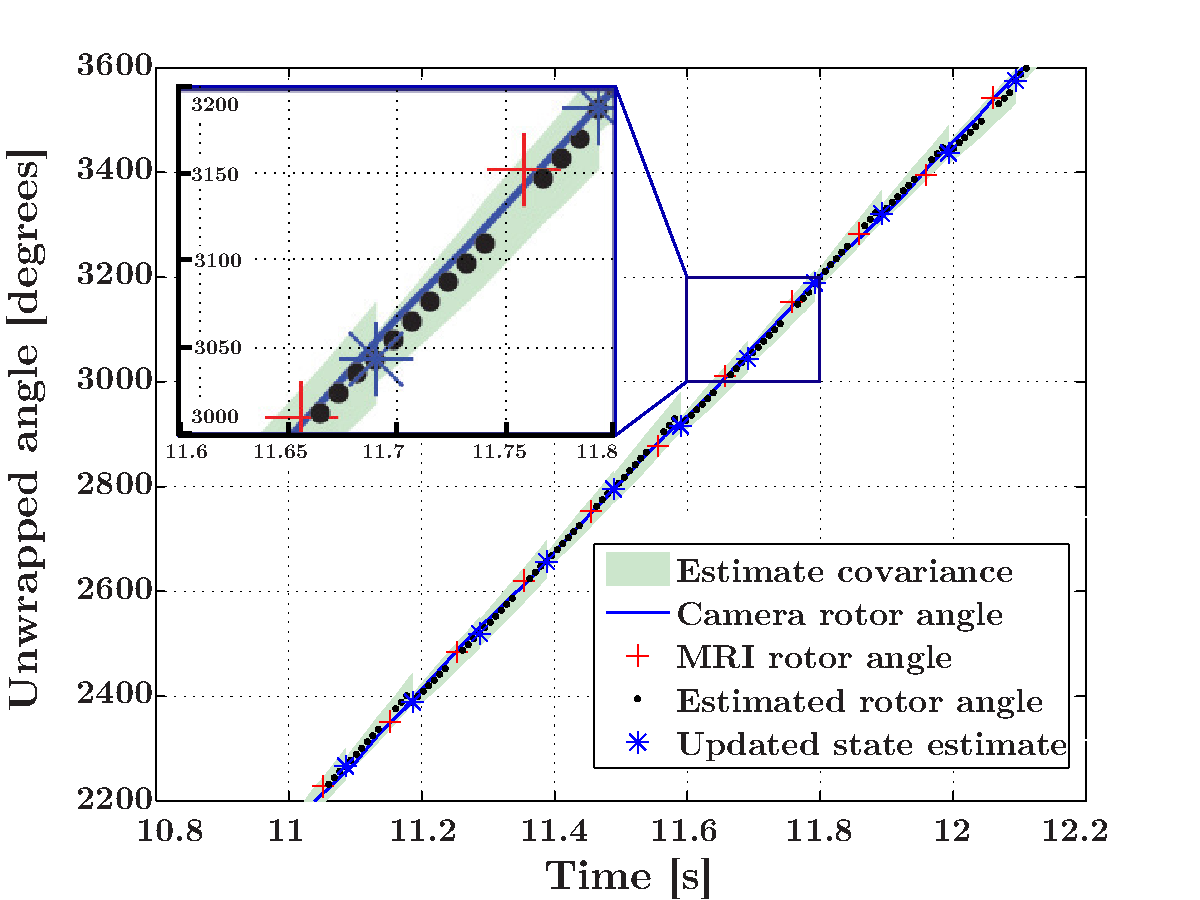
\includegraphics[width=1.0\columnwidth]{Figure13.pdf}
\end{center}
\caption{MRI-based estimation of rotor angle versus video camera measurements. Estimator variance is illustrated by a shaded region of $\pm$1 standard deviation.}
\label{fig:Estimate-Performance-PlusZoom}
\vspace{-5pt}
\end{figure}

\subsection{Maximum Torque Control}\label{subsec:ExpMaxTorque}

Closed-loop commutation was used to measure the maximum output torque, or stall torque, that the actuator could stably produce. For these experiments, the scalar control input, $u(t)$, in \eqref{eq:ControlLaw} was set to the magnitude of the maximum gradient of the scanner, $g_M$. For the Siemens Skyra scanner, this results in $u(t)=g_M=\pm 23$mT/m. By pulling against the set of  calibrated MR-compatible NiTi springs ($k = 215\frac{\textnormal{N}}{\textnormal{m}}$) depicted in Fig.\ \ref{fig:experimental-setup}, it was possible to evaluate the maximum potential needle force that could be applied by the actuator. 

\begin{figure}[b]
\begin{center}
	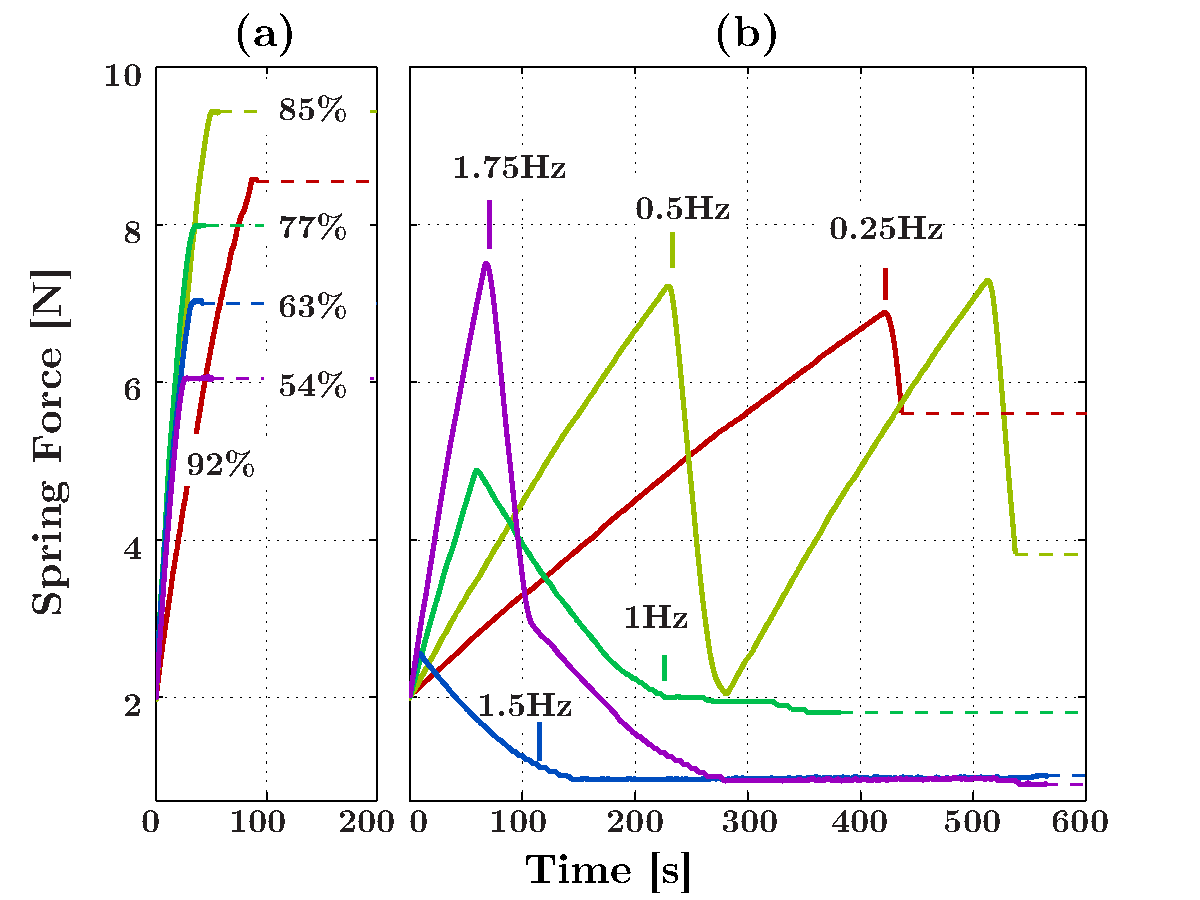
\includegraphics[width=1.0\columnwidth]{Figure14.pdf}
\end{center}
\caption{Spring force versus time for MRI actuation starting at $t$=0. (a) Closed-loop commutation. Labels express actuation duty cycle as a percentage. (b) Open-loop commutation. Labels indicate input frequency. Dashed lines in (a) and (b) indicate steady-state spring extension.} 
\label{fig:force-experiments}
\end{figure}

\begin{figure*}[]
\begin{center}
	\subfigure[]{
		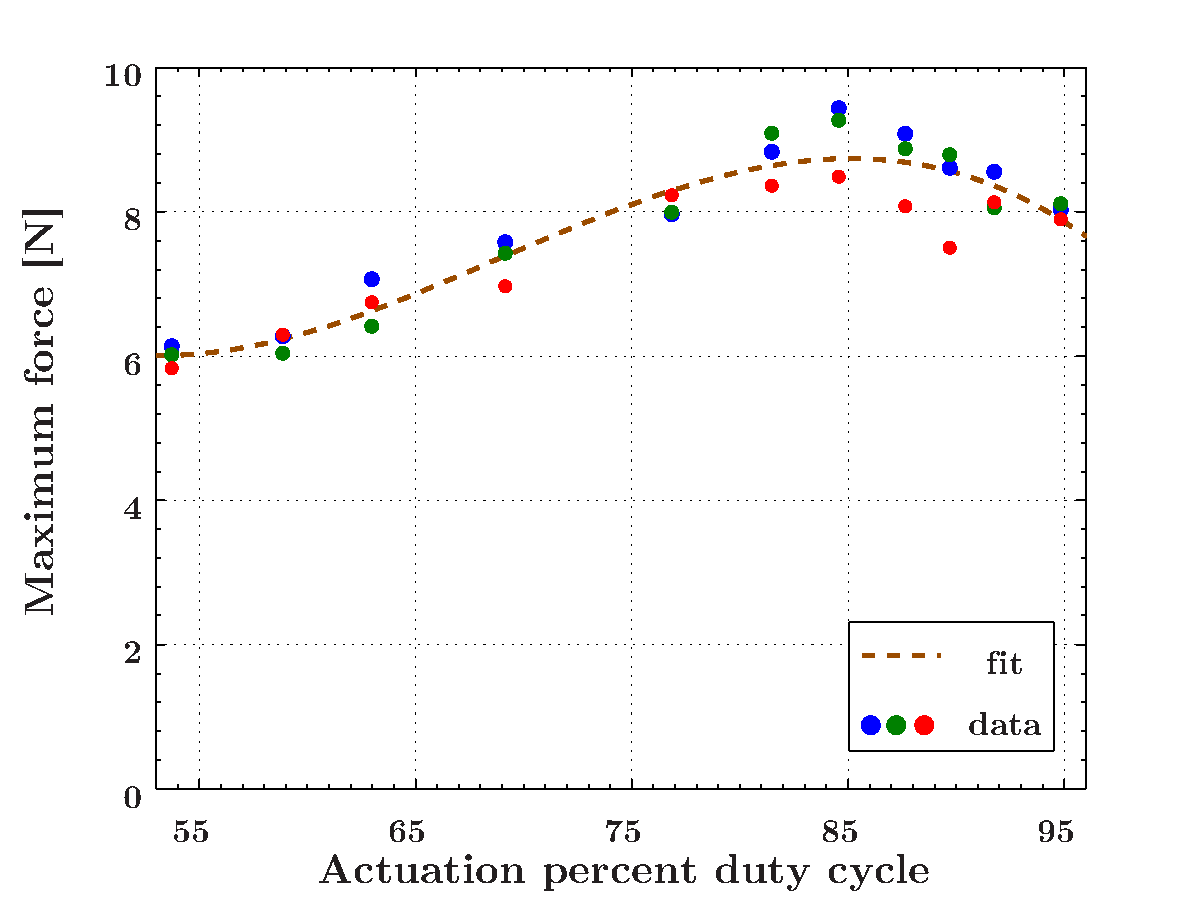
\includegraphics[width=0.89\columnwidth]{Figure15a.pdf}
		\label{fig:max-force-closedLoop}
	}
	\subfigure[]{
		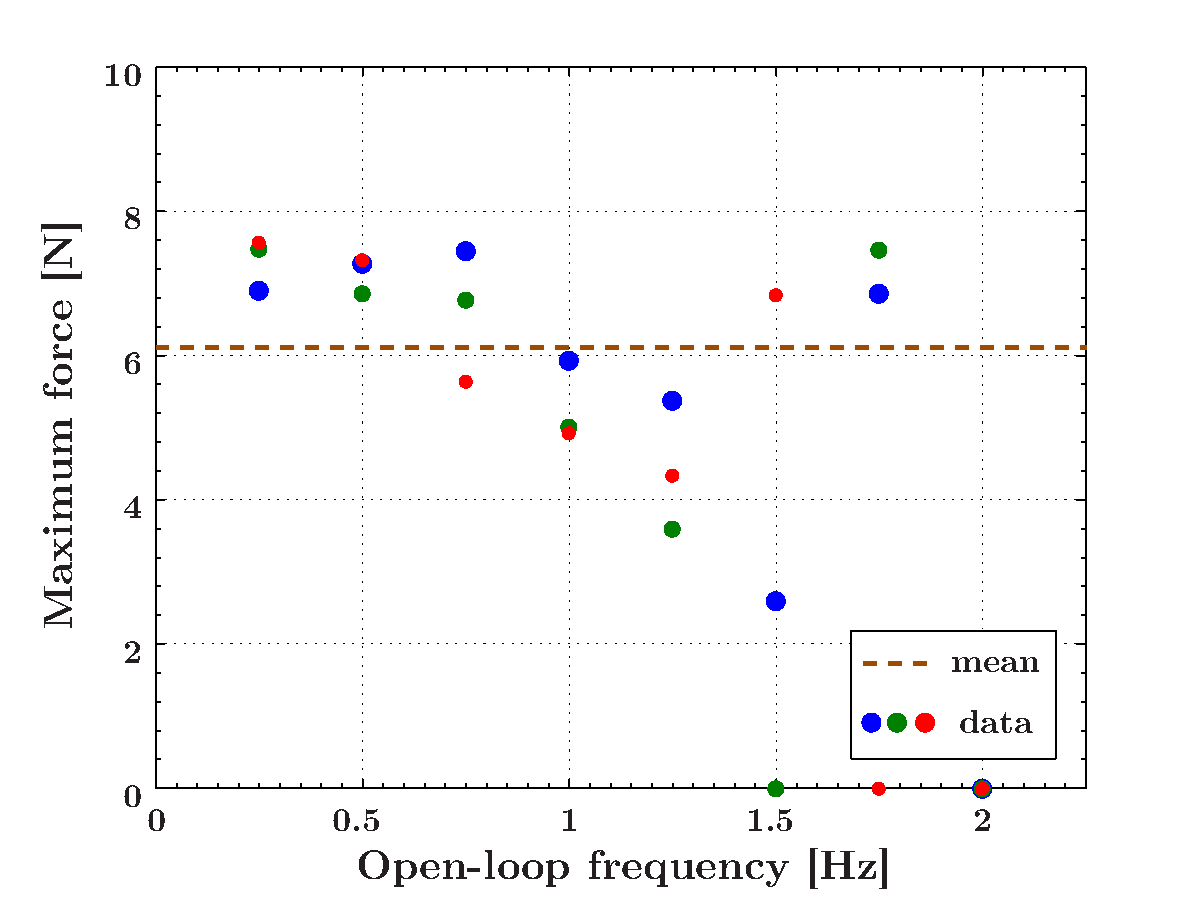
\includegraphics[width=0.89\columnwidth]{Figure15b.pdf}	
		\label{fig:max-force-OpenLoop}
	}
\end{center}
\caption{\label{fig:max-force-both}
Maximum spring force during closed- and open-loop commutation. Three trials are shown for each input value.
(a) Closed-loop maximum force versus actuation duty cycle. 
(b) Open-loop maximum force versus input frequency.}
\vspace{-5pt}
\end{figure*}


\begin{figure}
\begin{center}
	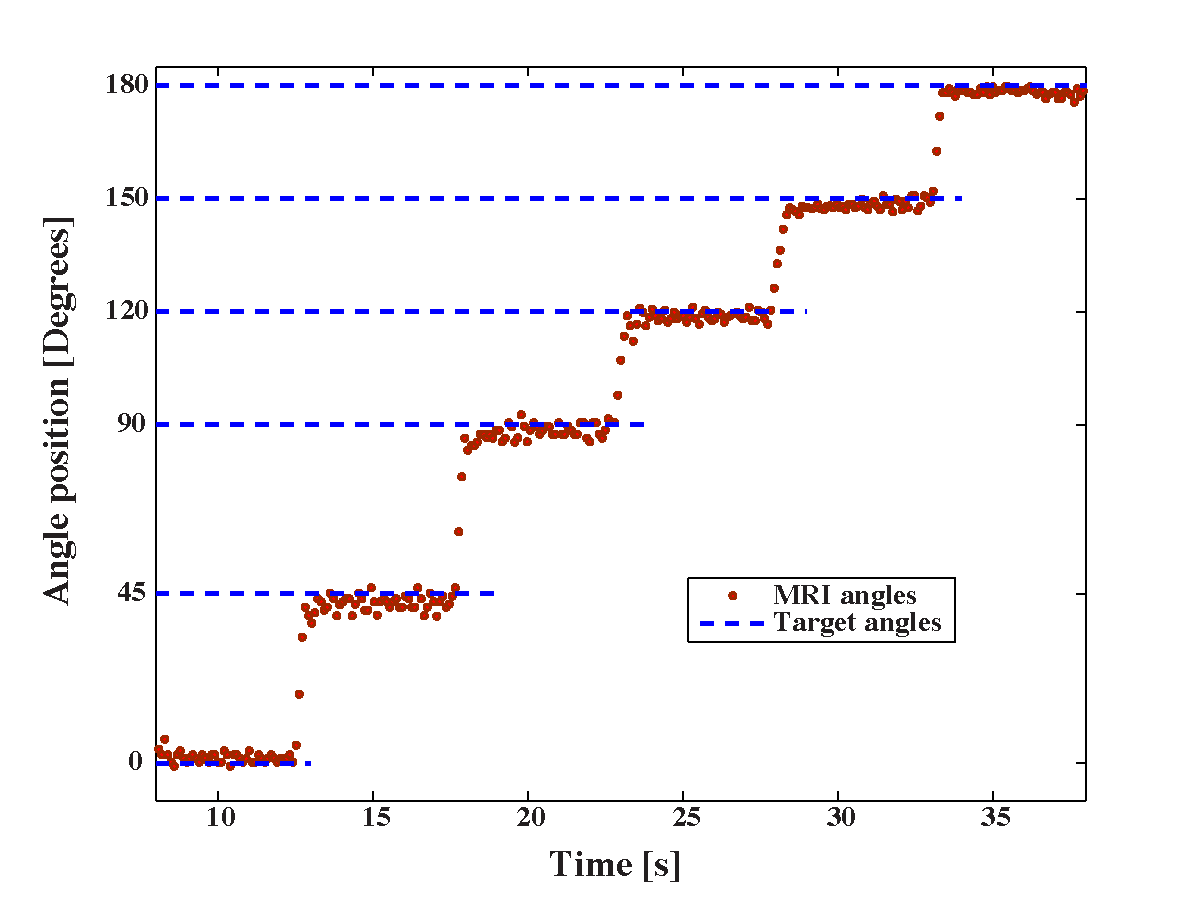
\includegraphics[width=1.0\columnwidth]{Figure16.pdf}
\end{center}
\caption{Regulation of rotor angle. Step responses using PID control for target angles = \{$0^\circ$, $45^\circ$, $90^\circ$, $120^\circ$, $150^\circ$, $180^\circ$\}.}
\label{fig:pid1-results}
\vspace{-10pt}
\end{figure}


Recall from Fig. \ref{fig:timing-diagram} that the overall pulse sequence includes a variable length actuation sequence. Increasing the length of this actuation sequence increases the relative amount of time spent actuating versus imaging the rotor. This decreases the rotor angle measurement rate, however, resulting in a less accurate estimate of rotor angle. To investigate this tradeoff, experiments were performed for a set of 11 actuation durations, $t_{act}$.  Results are reported in terms of duty cycle, $\frac{t_\textnormal{act}}{t_\textnormal{act}+t_\textnormal{off}}$, where $t_\textnormal{{off}}$ is defined as imaging time + 0.5ms to account for the ramp up and ramp down time of the actuation gradient.

To provide a comparison with prior work, open-loop commutation experiments were also performed. In these experiments, an open-loop sinusoidal gradient force of frequency $\omega$ was applied to the rotor, 
\begin{align}
\begin{bmatrix}F_x\\F_y\\F_z\end{bmatrix} =  g_M
\begin{bmatrix}
-\sin \omega t \\ 
0 \\ 
\cos \omega t \end{bmatrix}
\label{eq:openLoopControlLaw}
\end{align}
Starting from arbitrary initial conditions, the rotor is able to synchronize with the applied gradient force under certain conditions. Experiments were performed using eight input frequencies, $\omega$.



Three trials were run for each controller configuration. Representative trials of closed- and open-loop commutation are presented in Fig.\ \ref{fig:force-experiments}. The depicted closed-loop trials correspond to $t_\textnormal{act} = \{40, 50, 80, 120, 225\}\,$ms while the open-loop trials are for $\omega/2\pi = \{0.25, 0.5, 1, 1.5, 1.75\}\,$Hz. With closed-loop control, the actuator rotates at high velocity ($\sim$10Hz) that gradually decreases with an increasing load until the stall force is reached. In contrast, open-loop commutation results in lower forces attained over significantly longer time periods. 

Furthermore, in open loop, the rotor often slips, i.e., falls out of synchrony with the rotating gradient force. Since the actuator is backdrivable, any spring force at the time of slip can cause the rotor to rotate rapidly in the reverse direction. This phenomena can be observed in all the depicted open-loop trials. As the spring relaxes, the rotor sometimes resynchronizes with the applied gradient and again produces an increasing spring force. Such a situation is depicted for $\omega/2\pi=0.5$Hz. Alternately, the rotor may enter an oscillating limit cycle that results in a nonzero, but small, steady-state force, as illustrated by the plot for $\omega/2\pi=1.5$Hz.

The maximum forces for all open- and closed-loop trials are shown in Fig. \ref{fig:max-force-both}. Closed-loop control attains higher maximum forces and is up to twice as fast as the best open-loop control. In closed-loop control, the maximum force occurs for $t_\textnormal{act} = 120\,$ms corresponding to an 84.6\% duty cycle. Note that rotor slipping was never observed in closed loop. Thus, these maximum forces are true stall forces that can be applied indefinitely. In open loop, reverse rotor motion always followed the force peak due to desynchronization and actuator backdrivability. It can also be observed that, for open-loop input frequencies above 1Hz, the variation in maximum force increases and, for 1.5Hz and higher, the rotor sometimes failed to synchronize with the input gradient and so did not produce any force.



\subsection{Closed-Loop Position Control}
\label{subsec:ExpClosedLoopPositionControl}

Closed-loop commutation also makes it possible to regulate rotor angle to desired values. To investigate this, a PID position controller was implemented through \eqref{eq:ControlLaw}. Given a desired position $\theta_{\textrm{goal}}$, the control input is expressed in terms of position error, $e(t)$, the maximum gradient, $g_M$, at which the control input saturates, and the PID gains, $\{K_p, K_i, K_d\}$,
   \begin{align}
e(t) &=\theta_{\textrm{goal}} - \theta(t)\nonumber \\
\bar{u}(t) &= K_{p}  e(t) + K_i\int_0^t e(\tau) - K_d \dot{\theta}(t) \nonumber \\
u(t) &= \begin{cases}
   +g_{M} & \text{if } \bar{u}(t) > +g_{M}   \\
   \bar{u}(t) & \text{if } -g_M \le \bar{u}(t) \le +g_{M}   \\
   -g_{M}      & \text{if } \bar{u}(t)  < -g_{M} 
  \end{cases}
\label{eq:positioncontrol}
   \end{align}

For these trials, the actuator of Fig. \ref{fig:experimental-setup} was used with the springs disconnected such that the load consisted of transmission friction and inertia. The parameters $\{K_p, K_i, K_d\}$ were tuned manually ($K_{p} = 0.01\frac{T}{m.rad}$, $K_d = 0.011\frac{T.s}{m.rad}$, $K_i = 0.016\frac{T}{m.rad}$). Fig.\ \ref{fig:pid1-results} illustrates the step response for six commanded angles. Mean steady-state position error lies within the $\pm2^\circ$ resolution of the tracking algorithm.  


\subsection{Imaging Artifacts due to Actuator}
\label{subsec:ExpClosedLoopPositionControl}
\begin{figure}
\begin{center}
	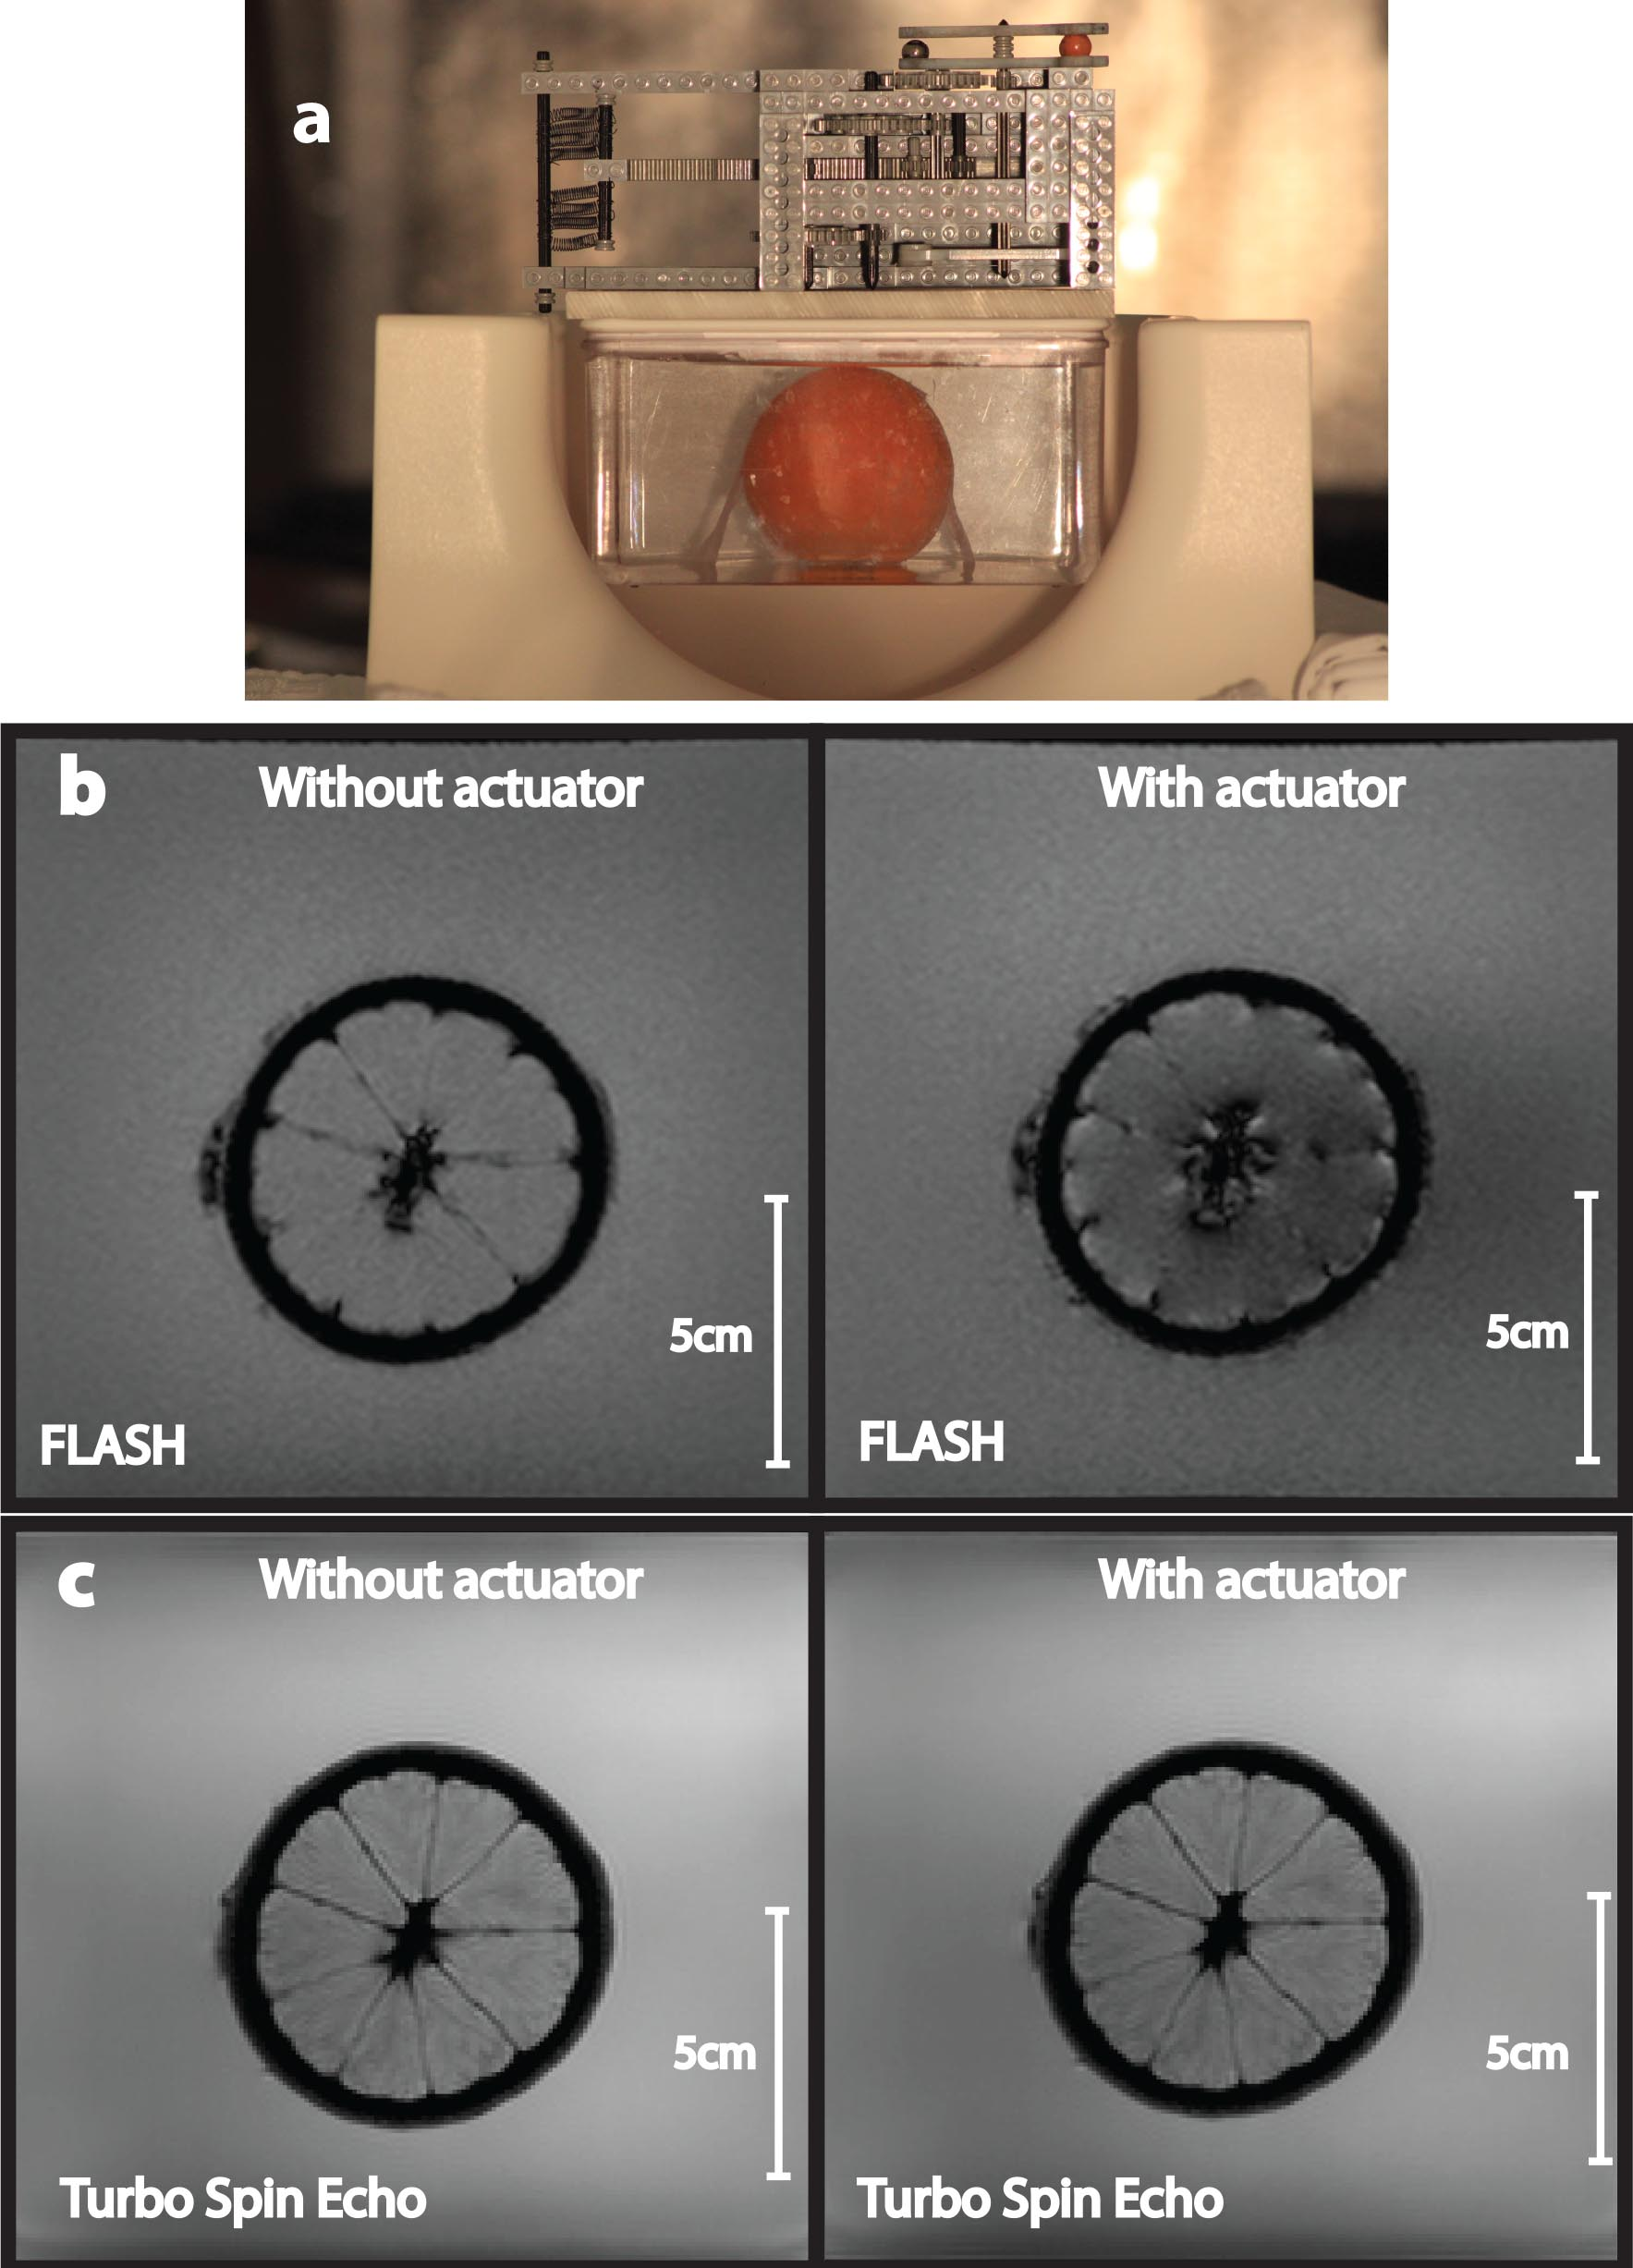
\includegraphics[width=1.0\columnwidth]{Figure17.jpg}
\end{center}
\caption{Effect of actuator on MR imaging. 
(a) Actuator placed above phantom consisting of an orange in a tank of water. Images consist of a coronal slice through the middle of the orange.
(b) Gradient echo FLASH sequence (TR/TE=8.6/4ms, slice thickness=4mm, number of averages 2, flip angle=20$^\circ$, FOV=218mm, base resolution=512) shows imaging artifacts.
(c)  Fast spin echo imaging (TR/TE=4000/77ms, slice thickness=4mm, Echo train length=13, number of averages 2, flip angle=150$^\circ$, FOV=218mm, base resolution=256) is insensitive to presence of actuator.
 \label{fig:artifact}}
\end{figure}

The induced magnetic field of the ferromagnetic material in the actuator perturbs the homogeneity of the $B_0$ static field of the scanner. This  creates image artifacts consisting of dark spots due to signal loss as well as geometrical distortions. The most important factors affecting artifact severity are (1) the distance between the ferrous particle and the imaging region and (2) the imaging sequence and its parameters \cite{Posse1990Susceptibility}. 

To assess image artifacts created by the actuator, a sequence of MR images were taken of an orange in a water tank with and without the actuator. As shown in Fig. \ref{fig:artifact}, the actuator was placed above the orange such that the ferrous particle was as close as possible to the orange and consequently would generate the most severe artifact. This configuration could correspond to the actuator placed on the torso of a patient. For all MR imaging, the camera used to take Fig. \ref{fig:artifact} was left in position outside the 5-Gauss line of the scanner. 

The first set of images shown in Fig. \ref{fig:artifact}(b) use a FLASH (Fast Low Angle SHot) sequence, which is known to be sensitive to imaging artifacts. The effect of the actuator on the image can be clearly seen. As shown in Fig. \ref{fig:artifact}(c), these artifacts can be virtually eliminated, however, by replacing the FLASH sequence with a fast spin echo sequence, which is more robust to magnetic field distortions. 

\section{Conclusions}
\label{sec:conclusions}

MRI-powered actuators constitute a new actuation technology for MR-guided robotic interventions. Since these devices can be fabricated from inexpensive materials, are tetherless and their control is accomplished entirely through scanner programming, this technology may enable new MR-guided interventions as well as facilitate current procedures. For example, the 9.4N maximum forces demonstrated here would be sufficient for in vivo human prostate capsule puncture during brachytherapy (8.9 N maximum force reported using 18G needles~\cite{podder2006vivo}).

Since this approach differs fundamentally from traditional MRI programming, its development poses interesting and challenging engineering problems. This paper addressed several fundamental challenges. First, it  proposed a new approach to track ferrous material by generating RF-selective signatures in properly located fiducial markers. Second,  it presented a technique to use tracking data to estimate the angular position and velocity of a moving rotor.  Third, it employed this estimate for closed-loop commutation control by interleaving imaging and actuation pulse sequences. Demonstrated benefits on a clinical MRI scanner include maximization of motor torque and velocity, avoidance of slip and regulation of motor angle.

There are a number of directions in which this work can be easily extended. For example, while the use of LEGO components facilitated prototype development, it can be anticipated that refined designs fabricated from precision components will yield even better results. Furthermore, while the algorithms were demonstrated here for a vertical rotor axis, counterbalancing the rotor enables rotation about any axis without the need for gravity compensation. In addition, if the actuator is mounted on a moving robot link, its commutation control could be achieved by tracking its rotor axis and location. Depending on robot design, this could be as simple as computing forward kinematics. Finally, for applications requiring simultaneous control of multiple actuators, promising control laws, such as that of \cite{becker2014simultaneously}, can be substituted for the feedback controllers presented here. 

\bibliographystyle{IEEEtran}
\bibliography{IEEEabrv,./bib/bibliography}

\begin{IEEEbiography}[{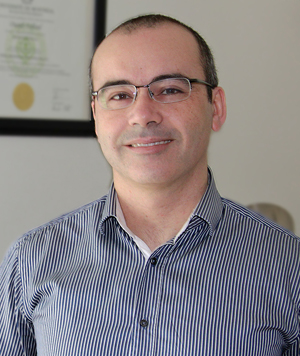
\includegraphics[width=1in,height=1.25in,clip,keepaspectratio]{Figures/OuajdiFelfoul.jpg}}]{Ouajdi Felfoul} received the M.S. and PhD degrees in biomedical engineering from Polytechnique Montreal (Canada), in 2005 and 2011. He is a Postdoctoral Research Fellow at the Pediatric Cardiac Bioengineering lab at the Boston Children’s Hospital where he is developing transformative robotic technology that utilizes Magnetic Resonance Imaging (MRI) systems to power, control and image robots under the guidance and control of a clinician.
\end{IEEEbiography}
\begin{IEEEbiography}[{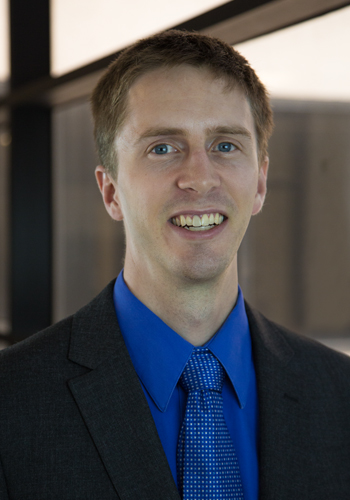
\includegraphics[width=1in,height=1.25in,clip,keepaspectratio]{Figures/AaronBecker.jpg}}]{Aaron Becker}
 (M`06) received M.S. and PhD degrees in electrical and computer engineering from the University of Illinois at Urbana-Champaign, in 2008 and 2012. He was a post doctoral research scholar at the Multi-Robot Systems Lab at Rice University and a post doctoral research fellow Boston Children's Hospital, Harvard Medical School, before joining the Electrical and Computer Engineering Department at the University of Houston as an Assistant Professor. His main research interests include controlling robots using uniform control inputs.
\end{IEEEbiography}
\begin{IEEEbiography}[{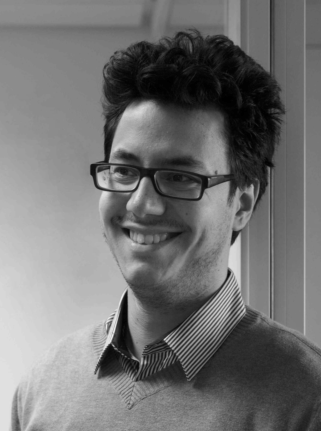
\includegraphics[width=1in,height=1.25in,clip,keepaspectratio]{Figures/ChristosBergeles.png}}]{Christos Bergeles}
 (M`11) received the M.Sc. degree in electrical and computer engineering from the National Technical University of Athens, Greece, in 2006, and the Ph.D. degree in mechanical engineering from ETH Zurich, Zurich, Switzerland, in 2011. He was a post doctoral research fellow at Boston Children's Hospital, Harvard Medical School, before joining the Hamlyn Centre for Robotic Surgery, Imperial College London as a Hamlyn Fellow. His main research interests include miniaturized telesurgical robotic platforms and medical image processing for robot guidance.
\end{IEEEbiography}
\begin{IEEEbiography}[{
\includegraphics[width=1in,height=1.25in,clip,keepaspectratio]{Figures/DupontPierre.jpg}}]{Dupont Pierre}
Pierre E. Dupont (M’99–SM’03–F’11) received the B.S., M.S., and Ph.D. degrees in mechanical engineering from Rensselaer Polytechnic Institute, Troy, NY, in 1982, 1984, and 1988, respectively.
From 1988 to 1990, he was a Postdoctoral Fellow with the School of Engineering and Applied Sciences, Harvard University, Cambridge, MA. He was a Professor of Mechanical Engineering and Biomedical Engineering with Boston University, Boston, MA. He is currently the Chief of Pediatric Cardiac Bioengineering with Boston Children's Hospital, Harvard Medical School, Boston, where he is engaged in developing instrumentation and imaging technology for minimally invasive surgery.
\end{IEEEbiography}

\end{document}
